\flushbottom


%% CONTINUE
%% Show that the solutions to a first order differential equation are a 
%% one-parameter family.




%%=============================================================================
%%=============================================================================
\chapter{First Order Differential Equations}
\label{chapter_foo}
\index{differential equations!first order}

Don't show me your technique.  Show me your heart.

\begin{flushright}
  -Tetsuyasu Uekuma
\end{flushright}








%%=============================================================================
\section{One Parameter Families of Functions}



Consider the equation:
\begin{equation}
  \label{equation F(x,y(x),c)=0}
  F(x, y(x), c) = 0,
\end{equation}
which implicitly defines a one-parameter family of functions $y(x;c)$.
Here $y$ is a function of the variable $x$ and the parameter $c$.
For simplicity, we will write $y(x)$ and not explicitly show the 
parameter dependence.


\begin{Example}
  The equation $y = c x$ defines family of lines with slope $c$, passing
  through the origin.  The equation $x^2 + y^2 = c^2$ defines circles
  of radius $c$, centered at the origin.

  Consider a 
  \hyperref[chapter spherical chicken]{chicken}
  dropped from 
  a height $h$.  The elevation $y$ of the chicken at time $t$ after 
  its release is $y(t) = h - g t^2$, where $g$ is the acceleration due 
  to gravity.  This is family of functions for the parameter $h$.
\end{Example}


It turns out that the general solution of any first order differential
equation is a one-parameter family of functions.  This is not easy to
prove.  However, it is easy to verify the converse.
We differentiate Equation~\ref{equation F(x,y(x),c)=0} with respect 
to $x$.
\[
F_x + F_y y' = 0
\]
(We assume that $F$ has a non-trivial dependence on $y$, that is $F_y
\neq 0$.)  This gives us two equations involving the independent
variable $x$, the dependent variable $y(x)$ and its derivative and the
parameter $c$.  If we algebraically eliminate $c$ between the two
equations, the eliminant will be a first order differential equation
for $y(x)$.  Thus we see that every one-parameter family of functions
$y(x)$ satisfies a first order differential equation.  This $y(x)$ is
the \textit{primitive} of the differential equation.  Later we will
discuss why $y(x)$ is the \textit{general solution} of the
differential equation.
%% CONTINUE  add a link for ``Later'' if I do show that.




\begin{Example}
  Consider the family of circles of radius $c$ centered about the origin.
  \[
  x^2 + y^2 = c^2
  \]
  Differentiating this yields:
  \[
  2 x + 2 y y' = 0.
  \]
  It is trivial to eliminate the parameter and obtain a differential equation
  for the family of circles.
  \[
  x + y y' = 0
  \]
  We can see the geometric meaning in this equation by writing it in the 
  form:
  \[
  y' = - \frac{x}{y}.
  \]
  For a point on the circle, the slope of the tangent $y'$
  is the negative of the cotangent of the angle $x/y$.
  (See Figure~\ref{figure circle tangent}.)
  \begin{figure}[tb!]
    \begin{center}
      %% CONTINUE Fix this graphic.
      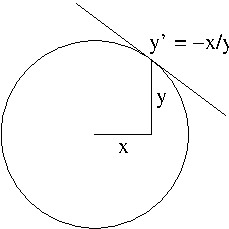
\includegraphics[width=0.2\textwidth]{ode/first_order/circle_tangent}
    \end{center}
    \caption{A circle and its tangent.}
    \label{figure circle tangent}
  \end{figure}
\end{Example}




\begin{Example}
  Consider the one-parameter family of functions:
  \[
  y(x) = f(x) + c g(x),
  \]
  where $f(x)$ and $g(x)$ are known functions.  The derivative is
  \[
  y' = f' + c g'.
  \]
  We eliminate the parameter.
  \begin{gather*}
    g y' - g' y = g f' - g' f \\
    y' - \frac{g'}{g} y = f' - \frac{g' f}{g}
  \end{gather*}
  Thus we see that $y(x) = f(x) + c g(x)$ satisfies a first order 
  \textit{linear} differential equation.  Later we will prove the 
  converse: the general solution of a first order linear differential
  equation has the form: $y(x) = f(x) + c g(x)$.
\end{Example}



We have shown that every one-parameter family of functions satisfies a first 
order differential equation.  We do not prove it here, but the converse 
is true as well.


\begin{Result}
  Every first order differential equation has a one-parameter family of 
  solutions $y(x)$ defined by an equation of the form:
  \[
  F(x, y(x); c) = 0.
  \]
  This $y(x)$ is called the \textit{general solution}.  If the
  equation is linear then the general solution expresses the
  totality of solutions of the differential equation.  If the
  equation is nonlinear, there may be other special \textit{singular
    solutions}, which do not depend on a parameter.
\end{Result}



This is strictly an existence result.  It does not say that the general 
solution of a first order differential equation can be determined by some
method, it just says that it exists.  There is no method for solving 
the general first order differential equation.  However, there are some
special forms that are soluble.  We will devote the rest of this chapter 
to studying these forms.





%%=============================================================================
\section{Integrable Forms}


In this section we will introduce a few forms of differential equations
that we may solve through integration.


%%-----------------------------------------------------------------------------
\subsection{Separable Equations}
\index{differential equations!separable}
\index{separable equations}




Any differential equation that can written in the form
\[ 
P(x) + Q(y) y' = 0
\]
is a \textit{separable equation}, (because the dependent and independent
variables are separated).  We can obtain an implicit solution by integrating
with respect to $x$.
\begin{gather*}
  \int P(x) \,\dd x + \int Q(y) \frac{\dd y}{\dd x} \,\dd x = c 
  \\
  \int P(x) \,\dd x + \int Q(y) \,\dd y = c
\end{gather*}



\begin{Result}
  The separable equation $P(x) + Q(y) y' = 0$ may be solved by integrating
  with respect to $x$.  The general solution is
  \[ 
  \int P(x) \,\dd x + \int Q(y) \,\dd y = c.
  \]
\end{Result}



\begin{Example}
  Consider the differential equation $y' = x y^2$.
  We separate the dependent and independent variables and integrate to find
  the solution.
  \begin{gather*}
    \frac{\dd y}{\dd x} = x y^2 
    \\
    y^{-2}\,\dd y = x\,\dd x 
    \\
    \int y^{-2}\,\dd y = \int x \,\dd x + c 
    \\
    -y^{-1} = \frac{x^2}{2} + c 
    \\
    \boxed{
      y = - \frac{1}{x^2/2 + c}
      }
  \end{gather*}
\end{Example}







\begin{Example}
  The equation $y' = y - y^2$ is separable.
  \[
  \frac{y'}{y - y^2} = 1
  \]
  We expand in partial fractions and integrate.
  \begin{gather*}
    \left( \frac{1}{y} - \frac{1}{y-1} \right) y' = 1 
    \\
    \ln |y| - \ln |y - 1| = x + c
  \end{gather*}
  We have an implicit equation for $y(x)$.  Now we solve for $y(x)$.
  \begin{gather*}
    \ln \left| \frac{y}{y-1} \right| = x + c 
    \\
    \left| \frac{y}{y-1} \right| = \e^{x+c} 
    \\
    \frac{y}{y-1} = \pm \e^{x+c} 
    \\
    \frac{y}{y-1} = c \e^x 
    \footnote{Here we have substituted $c$ for $\pm \e^c$.}
    \\
    y = \frac{c \e^x}{c \e^x - 1}
    \\
    \boxed{
      y = \frac{1}{1 + c \e^{x}}
      }
  \end{gather*}
\end{Example}










%%=============================================================================
\subsection{Exact Equations}
\index{differential equations!exact}
\index{exact equations}



Any first order ordinary differential equation of the first degree can 
be written as the total differential equation,
\[
P(x, y) \,\dd x + Q(x, y) \,\dd y = 0.
\]
If this equation can be integrated directly, that is if there is a primitive,
$u(x, y)$, such that 
\[
d u = P \,\dd x + Q \,\dd y,
\]
then this equation is called \textit{exact}.
The (implicit) solution of the differential equation is 
\[
u(x, y) = c,
\]
where $c$ is an arbitrary constant.  
Since the differential of a function, $u(x, y)$, is
\[
\dd u \equiv \frac{\partial u}{\partial x} \,\dd x + \frac{\partial u}{\partial y} \,\dd y,
\]
$P$ and $Q$ are the partial derivatives of $u$:
\[
P(x, y) = \frac{\partial u}{\partial x}, \qquad 
Q(x, y) = \frac{\partial u}{\partial y}.
\]

In an alternate notation, the differential equation
\begin{equation}
  \label{first_order_first_degree}
  P(x, y) + Q(x, y) \frac{\dd y}{\dd x} = 0,
\end{equation}
is exact if there is a primitive $u(x, y)$ such that
\[
\frac{\dd u}{\dd x} \equiv \frac{\partial u}{\partial x} + \frac{\partial u}{\partial y} \frac{\dd y}{\dd x}
= P(x, y) + Q(x, y) \frac{\dd y}{\dd x}.
\]
The solution of the differential equation is $u(x, y) = c$.





\begin{Example}
  \[
  x + y \frac{\dd y}{\dd x} = 0
  \]
  is an exact differential equation since
  \[
  \frac{\dd}{\dd x} \left( \frac{1}{2} (x^2 + y^2) \right) = x + y \frac{\dd y}{\dd x}
  \]
  The solution of the differential equation is
  \[
  \frac{1}{2} (x^2 + y^2) = c.
  \]
\end{Example}




\begin{Example}
  \label{product_rule_exact_equation},
  Let $f(x)$ and $g(x)$ be known functions.
  \[
  g(x) y' + g'(x) y = f(x)
  \]
  is an exact differential equation since
  \[
  \frac{\dd}{\dd x} \left( g(x) y(x) \right) = g y' + g' y.
  \]
  The solution of the differential equation is
  \begin{gather*}
    g(x) y(x) = \int f(x)\,\dd x + c \\
    y(x) = \frac{1}{g(x)} \int f(x) \,\dd x + \frac{c}{g(x)}.
  \end{gather*}
\end{Example}



\paragraph{A necessary condition for exactness.}
The solution of the exact equation $P + Q y' = 0$ is $u = c$
where $u$ is the primitive of the equation,  $\frac{\dd u}{\dd x} = P + Q y'$.
At present the only method we have for determining the primitive is 
guessing.   This is fine for simple equations, but for more difficult
cases we would like a method more concrete than divine inspiration.  As a
first step toward this goal we determine a criterion for determining if
an equation is exact.

Consider the exact equation,
\[
P + Q y' = 0,
\]
with primitive $u$, where we assume that the functions $P$ and $Q$ are 
continuously differentiable.  Since the mixed partial derivatives of $u$ 
are equal,
\[
\frac{\partial^2 u}{\partial x \partial y} = \frac{\partial^2 u}{\partial y \partial x},
\]
a necessary condition for exactness is
\[
\frac{\partial P}{\partial y} = \frac{\partial Q}{\partial x}.
\]



\paragraph{A sufficient condition for exactness.}
This necessary condition for exactness is also a sufficient condition.
We demonstrate this by deriving the general solution of 
(\ref{first_order_first_degree}).  Assume that $P + Q y' = 0$
is not necessarily exact, but satisfies the condition $P_y = Q_x$.
If the equation has a primitive, 
\[
\frac{\dd u}{\dd x} \equiv \frac{\partial u}{\partial x} + \frac{\partial u}{\partial y} \frac{\dd y}{\dd x}
= P(x, y) + Q(x, y) \frac{\dd y}{\dd x},
\]
then it satisfies
\begin{equation}
  \label{ux=p_uy=q}
  \frac{\partial u}{\partial x} = P, \qquad \frac{\partial u}{\partial y} = Q.
\end{equation}
Integrating the first equation of (\ref{ux=p_uy=q}), we see that the 
primitive has the form
\[
u(x, y) = \int_{x_0}^x P(\xi, y) \,\dd \xi + f(y),
\]
for some $f(y)$.
Now we substitute this form into the second equation of (\ref{ux=p_uy=q}).
\begin{gather*}
  \frac{\partial u}{\partial y} = Q(x, y) \\
  \int_{x_0}^x P_y(\xi, y) \,\dd \xi + f'(y) = Q(x, y) \\
  \intertext{Now we use the condition $P_y = Q_x$.}
  \int_{x_0}^x Q_x(\xi, y) \,\dd \xi + f'(y) = Q(x, y) \\
  Q(x,y) - Q(x_0, y) + f'(y) = Q(x, y) \\
  f'(y) = Q(x_0, y) \\
  f(y) = \int_{y_0}^y Q(x_0, \psi) \,\dd \psi
\end{gather*}
Thus we see that 
\[
u = \int_{x_0}^x P(\xi, y) \,\dd \xi + \int_{y_0}^y Q(x_0, \psi) \,\dd \psi
\]
is a primitive of the derivative; the equation is exact.  The solution of
the differential equation is
\[
\int_{x_0}^x P(\xi, y) \,\dd \xi + \int_{y_0}^y Q(x_0, \psi) \,\dd \psi = c.
\]
Even though there are three arbitrary constants: $x_0$, $y_0$ and $c$, 
the solution is a one-parameter family.  This is because changing 
$x_0$ or $y_0$ only changes the left side by an additive constant.




\begin{Result}
  Any first order differential equation of the first degree can be written
  in the form
  \[
  P(x, y) + Q(x, y) \frac{\dd y}{\dd x} = 0.
  \]
  This equation is exact if and only if
  \[
  P_y = Q_x.
  \]
  In this case the solution of the differential equation is given by
  \[
  \int_{x_0}^x P(\xi, y) \,\dd \xi 
  + \int_{y_0}^y Q(x_0, \psi) \,\dd \psi = c.
  \]
\end{Result}





%% CONTINUE: cover integrating factors.






%% Solve first order equations by inspection.
\begin{Exercise}
  \label{exercise gygyf}
  Solve the following differential equations by inspection.  That is, group 
  terms into exact derivatives and then integrate. 
  $f(x)$ and $g(x)$ are known functions.
  \begin{enumerate}
    %%
  \item $\frac{y'(x)}{y(x)} = f(x)$
    %%
  \item $y^\alpha(x) y'(x) = f(x)$
    %%
  \item $\frac{y'}{\cos x} + y \frac{\tan x}{\cos x} = \cos x$
  \end{enumerate}

  \hintsolution{gygyf}
\end{Exercise}























%%-----------------------------------------------------------------------------
\subsection{Homogeneous Coefficient Equations}
\index{differential equations!homogeneous coefficient}
\index{homogeneous coefficient equations}
\index{homogeneous functions}
\index{Euler's theorem}



Homogeneous coefficient, first order differential equations form another class
of soluble equations.  We will find that a change of dependent variable 
will make such equations separable or we can determine an integrating factor 
that will make such equations exact.  First we define homogeneous functions.



\paragraph{Euler's Theorem on Homogeneous Functions.}
The function $F(x,y)$ is \textit{homogeneous of degree} $n$ if
\[
F(\lambda x,\lambda y) = \lambda^n F(x,y).
\]
From this definition we see that
\[
F(x,y) = x^n F \left( 1, \frac{y}{x} \right).
\]
(Just formally substitute $1/x$ for $\lambda$.)
For example, 
\[
x y^2, \qquad
\frac{x^2 y+ 2 y^3}{x + y}, \qquad
x \cos(y/x)
\]
are homogeneous functions of orders 3, 2 and 1, respectively.


Euler's theorem for a homogeneous function of order $n$ is:
\[
x F_x + y F_y = n F.
\]
To prove this, we define $\xi = \lambda x$, $\psi = \lambda y$.
From the definition of homogeneous functions, we have
\[
F(\xi, \psi) = \lambda^n F(x,y).
\]
We differentiate this equation with respect to $\lambda$.
\begin{gather*}
  \frac{\partial F(\xi,\psi)}{\partial \xi} \frac{\partial \xi}{\partial \lambda}
  + \frac{\partial F(\xi,\psi)}{\partial \psi} \frac{\partial \psi}{\partial \lambda}
  = n \lambda^{n-1} F(x,y) \\
  x F_\xi + y F_\psi = n \lambda^{n-1} F(x,y)
\end{gather*}
Setting $\lambda = 1$, (and hence $\xi = x$, $\psi = y$),
proves Euler's theorem.


\begin{Result}
  \textbf{Euler's Theorem on Homogeneous Functions.}
  If $F(x, y)$ is a homogeneous function of degree $n$, then
  \[
  x F_x + y F_y = n F.
  \]
\end{Result}








\paragraph{Homogeneous Coefficient Differential Equations.}
If the coefficient functions $P(x, y)$ and $Q(x, y)$ are homogeneous of 
degree $n$ then the differential equation,
\begin{equation}
  \label{homogeneous differential equation}
  P(x, y) + Q(x, y) \frac{\dd y}{\dd x} = 0,
\end{equation}
is called a \textit{homogeneous coefficient equation}.  They are often
referred to simply as \textit{homogeneous equations}.   



\paragraph{Transformation to a Separable Equation.}
We can write the homogeneous equation in the form,
\begin{gather*}
  x^n P \left(1, \frac{y}{x} \right) 
  + x^n Q \left(1, \frac{y}{x} \right) \frac{\dd y}{\dd x} = 0, 
  \\
  P \left(1, \frac{y}{x} \right) 
  + Q \left(1, \frac{y}{x} \right) \frac{\dd y}{\dd x} = 0.
\end{gather*}
This suggests the change of dependent variable $u(x) = \frac{y(x)}{x}$.
\[
P(1, u) + Q(1, u) \left( u + x \frac{\dd u}{\dd x} \right) = 0
\]
This equation is separable.
\begin{gather*}
  P(1, u) + u Q(1, u) + x Q(1, u) \frac{\dd u}{\dd x} = 0 
  \\
  \frac{1}{x} + \frac{Q(1, u)}{P(1, u) + u Q(1, u)} \frac{\dd u}{\dd x} = 0 
  \\
  \ln |x| + \int \frac{1}{u + P(1, u) / Q(1, u)} \,\dd u = c 
  \\
  \intertext{By substituting $\ln |c|$ for $c$, we can write this in a 
    simpler form.}
  \int \frac{1}{u + P(1, u) / Q(1, u)} \,\dd u = \ln \left| \frac{c}{x} \right|.
\end{gather*}


\paragraph{Integrating Factor.}
One can show that
\[
\mu(x,y) = \frac{1}{x P(x,y) + y Q(x,y)}
\]
is an integrating factor for the Equation~
\ref{homogeneous differential equation}.  The proof of this is left as 
an exercise for the reader.  (See Exercise~
\ref{exercise integrating factor homogeneous}.)





\begin{Result}
  \textbf{Homogeneous Coefficient Differential Equations.}
  If $P(x, y)$ and $Q(x, y)$ are homogeneous functions of degree $n$, then
  the equation 
  \[
  P(x, y) + Q(x, y) \frac{\dd y}{\dd x} = 0
  \]
  is made separable by the change of independent variable 
  $u(x) = \frac{y(x)}{x}$.  The solution is determined by
  \[
  \int \frac{1}{u + P(1, u) / Q(1, u)} \,\dd u = \ln \left| \frac{c}{x} \right|.
  \]
  Alternatively, the homogeneous equation can be made exact with the 
  integrating factor
  \[
  \mu(x,y) = \frac{1}{x P(x,y) + y Q(x,y)}.
  \]
\end{Result}








\begin{Example}
  Consider the homogeneous coefficient equation
  \[
  x^2 - y^2 + x y \frac{\dd y}{\dd x} = 0.
  \]
  The solution for $u(x) = y(x) / x$ is determined by
  \begin{gather*}
    \int \frac{1}{u + \frac{1 - u^2}{u} }\,\dd u = \ln \left| \frac{c}{x} \right| 
    \\
    \int u \,\dd u = \ln \left| \frac{c}{x} \right| 
    \\
    \frac{1}{2} u^2 = \ln \left| \frac{c}{x} \right| 
    \\
    u = \pm \sqrt{2 \ln |c/x|}
  \end{gather*}
  Thus the solution of the differential equation is
  \[
  \boxed{
    y = \pm x \sqrt{2 \ln |c/x|}
    }
  \]
\end{Example}




%% CONTINUE: cover equations that are homogeneous and exact.
%% CONTINUE: integrating factor for homogeneous equations. 






%% \mu(x,y) = \frac{1}{x M(x,y) + y N(x,y)}
\begin{Exercise}
  \label{exercise integrating factor homogeneous}
  Show that
  \[
  \mu(x,y) = \frac{1}{x P(x,y) + y Q(x,y)}
  \]
  is an integrating factor for the homogeneous equation,
  \[
  P(x,y) + Q(x,y) \frac{\dd y}{\dd x} = 0.
  \]

  \hintsolution{integrating factor homogeneous}
\end{Exercise}







%% $d y / d t = f(y / t)$.
\begin{Exercise}[mathematica/ode/first\_order/exact.nb]
  \label{exercise dydt = f(y/t)}
  Find the general solution of the equation 
  \[
  \frac{\dd y}{\dd t} = 2 \frac{y}{t} + \left( \frac{y}{t} \right)^2.
  \]
  
  \hintsolution{dydt = f(y/t)}
\end{Exercise}











%%=============================================================================
\section{The First Order, Linear Differential Equation}
\index{differential equations!first order}



%%-----------------------------------------------------------------------------
\subsection{Homogeneous Equations}




The first order, linear, homogeneous equation has the form
\[ 
\frac{\dd y}{\dd x} + p(x) y = 0.
\]
Note that if we can find one solution, then any constant times that solution
also satisfies the equation.  In fact, all the solutions of this 
equation differ only by multiplicative constants.
We can solve any equation of this type because it is separable.
\begin{gather*}
  \frac{y'}{y} = - p(x) 
  \\
  \ln |y| = - \int p(x) \,\dd x + c 
  \\
  y = \pm \e^{- \int p(x) \,\dd x + c} 
  \\
  y = c \e^{- \int p(x) \,\dd x}
\end{gather*}




\begin{Result}
  \textbf{First Order, Linear Homogeneous Differential Equations.}
  The first order, linear, homogeneous differential equation,
  \[ 
  \frac{\dd y}{\dd x} + p(x) y = 0,
  \]
  has the solution
  \begin{equation}
    \label{first order linear homogeneous}
    y = c \e^{- \int p(x) \,\dd x}.
  \end{equation}
  The solutions differ by multiplicative constants.  
\end{Result}







\begin{Example}  
  Consider the equation
  \[ 
  \frac{\dd y}{\dd x} + \frac{1}{x} y = 0.
  \]
  We use Equation~\ref{first order linear homogeneous} to determine 
  the solution.
  \begin{gather*}
    y(x) = c \e^{ - \int 1/x \,\dd x }, \quad \mathrm{for}\ x \neq 0
    \\
    y(x) = c \e^{ - \ln |x| }
    \\
    y(x) = \frac{c}{|x|}
    \\
    \boxed{
      y(x) = \frac{c}{x}
      }
  \end{gather*}
\end{Example}
















%%-----------------------------------------------------------------------------
\subsection{Inhomogeneous Equations}






The first order, linear, inhomogeneous differential equation has the form
\begin{equation}
  \label{first_order_linear_inhomogeneous}
  \frac{\dd y}{\dd x} + p(x) y = f(x).
\end{equation}
This equation is not separable.  Note that it is similar to the exact equation
we solved in Example~\ref{product_rule_exact_equation},
\[
g(x) y'(x) + g'(x) y(x) = f(x).
\]
To solve Equation~\ref{first_order_linear_inhomogeneous}, 
we multiply by an \textit{integrating factor}.
\index{integrating factor}
Multiplying a differential equation by its integrating factor changes it to 
an exact equation.   Multiplying 
Equation~\ref{first_order_linear_inhomogeneous} by the function,
$I(x)$, yields,
\[
I(x) \frac{\dd y}{\dd x} + p(x) I(x) y = f(x) I(x).
\]
In order that $I(x)$ be an integrating factor, it must satisfy
\[
\frac{\dd}{\dd x} I(x) = p(x) I(x).
\]
This is a first order, linear, homogeneous equation with the solution
\[
I(x) = c \e^{\int p(x) \,\dd x}.
\]
This is an integrating factor for any constant $c$.  For simplicity we will
choose $c = 1$.




To solve Equation~\ref{first_order_linear_inhomogeneous} we
multiply by the integrating factor and integrate.
Let $P(x) = \int p(x)\,\dd x$.
\begin{gather*}
  \e^{P(x)} \frac{\dd y}{\dd x} + p(x) \e^{P(x)} y = \e^{P(x)}f(x) \\
  \frac{\dd}{\dd x} \left(\e^{P(x)} y \right) = \e^{P(x)}f(x) \\
  y = \e^{-P(x)}\int \e^{P(x)} f(x)\,\dd x + c \e^{-P(x)} \\
  y \equiv y_p + c \, y_h
\end{gather*}
Note that the \textit{general solution} is the sum of a  
\textit{particular solution}, $y_p$, that satisfies $y' + p(x) y = f(x)$,  
\index{particular solution}
and an arbitrary constant times a \textit{homogeneous solution}, 
\index{homogeneous solution}
$y_h$, that satisfies $y' + p(x) y = 0$.





\begin{Example}
  Consider the differential equation
  \[ 
  y' + \frac{1}{x} y = x^2, \quad x > 0. 
  \]
  First we find the integrating factor.
  \[ 
  I(x) = \exp \left( \int \frac{1}{x} \,\dd x \right) = \e^{\ln x} = x
  \]
  We multiply by the integrating factor and integrate.
  \begin{gather*}
    \frac{\dd}{\dd x} (x y) = x^3 
    \\
    x y = \frac{1}{4} x^4 + c 
    \\
    \boxed{ 
      y = \frac{1}{4} x^3 + \frac{c}{x}. 
      }
  \end{gather*}
  The particular and homogeneous solutions are
  \[ 
  y_p = \frac{1}{4} x^3 \qquad \mathrm{and} \qquad y_h = \frac{1}{x}. 
  \]
  Note that the general solution to the differential equation is a 
  one-parameter family of functions.  The general solution is plotted
  in Figure~\ref{figure one param} for various values of $c$.

  \begin{figure}[tb!]
    \begin{center}
      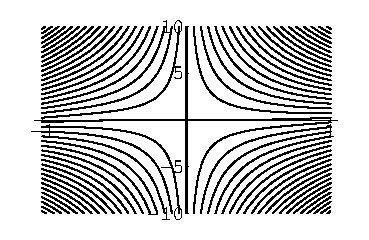
\includegraphics[width=0.4\textwidth]{ode/first_order/one_par}
    \end{center}
    \caption{The general solution for various values of the constant of
      integration.}
    \label{figure one param}
  \end{figure}

\end{Example}







%% y' - \frac{1}{x} y = x^\alpha.
\begin{Exercise}[mathematica/ode/first\_order/linear.nb]
  \label{exercise y - 1/x y = x alpha}
  Solve the differential equation
  \[
  y' - \frac{1}{x} y = x^\alpha, \quad x > 0.
  \]

  \hintsolution{y - 1/x y = x alpha}
\end{Exercise}







%%------------------------------------------------------------------------------
\subsection{Variation of Parameters.}
\index{variation of parameters!first order equation} 


We could also have found the particular solution with the method of 
variation of parameters. 
Although we can solve first order equations without this method, it will
become important in the study of higher order inhomogeneous equations.
We begin by assuming that the particular solution has the form 
$y_p = u(x) y_h(x)$ where $u(x)$ is an unknown function.  
We substitute this into the differential equation.
\begin{gather*}
  \frac{\dd}{\dd x} y_p + p(x) y_p = f(x) \\
  \frac{\dd}{\dd x} (u y_h) + p(x) u y_h = f(x) \\
  u' y_h + u (y_h' + p(x) y_h) = f(x) \\
  \intertext{Since $y_h$ is a homogeneous solution, $y_h' + p(x) y_h = 0$.}
  u' = \frac{f(x)}{y_h} \\
  u = \int \frac{f(x)}{y_h(x)}\,\dd x \\
  \intertext{Recall that the homogeneous solution is $y_h = \e^{-P(x)}$.}
  u = \int \e^{P(x)}f(x)\,\dd x
\end{gather*}
Thus the particular solution is
\[ 
y_p = \e^{-P(x)} \int \e^{P(x)}f(x)\,\dd x.
\]









%%=============================================================================
\section{Initial Conditions}
\index{initial conditions}




In physical problems involving first order differential equations, 
the solution satisfies both the differential equation and a constraint which 
we call the \textit{initial condition}.
Consider a first order linear differential equation subject to
the initial condition $y(x_0) = y_0$.  
The general solution is
\[ 
y = y_p + c y_h = \e^{-P(x)} \int \e^{P(x)} f(x) \,\dd x + c \e^{-P(x)}. 
\]
For the moment, we will assume that this problem is \textit{well-posed}.  
A problem is well-posed if there is a unique solution to the differential 
equation that satisfies the constraint(s).
Recall that $\int \e^{P(x)}f(x)\,\dd x$ denotes any integral of $\e^{P(x)} f(x)$.
For convenience, we choose $\int^x_{x_0} \e^{P(\xi)}f(\xi)\,\dd \xi$.  The initial
condition requires that
\[
y(x_0) = y_0 
= \e^{-P(x_0)}\int^{x_0}_{x_0} \e^{P(\xi)}f(\xi)\,\dd \xi + c \e^{-P(x_0)}
= c \e^{-P(x_0)}.
\]
Thus $c = y_0 \e^{P(x_0)}$. The solution subject to the initial condition is
\[
y = \e^{-P(x)}\int^x_{x_0} \e^{P(\xi)}f(\xi)\,\dd\xi + y_0 \e^{P(x_0)-P(x)}.
\]







\begin{Example}
  Consider the problem
  \[ 
  y' + (\cos x) y = x, \qquad y(0) = 2.
  \]
  From Result~\ref{first_order_inhom}, the solution subject to the initial 
  condition is
  \[ 
  \boxed{
    y = \e^{-\sin x} \int^x_0 \xi \e^{\sin \xi}\,\dd \xi + 2 \e^{-\sin x}.
    }
  \]
\end{Example}









%%-----------------------------------------------------------------------------
\subsection{Piecewise Continuous Coefficients and Inhomogeneities}


If the coefficient function $p(x)$ and the inhomogeneous term $f(x)$ in
the first order linear differential equation
\[ 
\frac{\dd y}{\dd x} + p(x) y = f(x) 
\]
are continuous, then the solution is continuous and has a continuous first 
derivative.   To see this, we note that the solution 
\[ 
y = \e^{-P(x)}\int \e^{P(x)}f(x)\,\dd x + c \e^{-P(x)}
\]
is continuous since the integral of a piecewise continuous function is
continuous.  The first derivative of the solution can be found directly
from the differential equation.
\[ 
y' = - p(x) y + f(x)
\]
Since $p(x)$, $y$, and $f(x)$ are continuous, $y'$ is continuous.

If $p(x)$ or $f(x)$ is only piecewise continuous, then the solution will be
continuous since the integral of a piecewise continuous function is continuous.
The first derivative of the solution will be piecewise continuous.






\begin{Example}
  Consider the problem
  \[ 
  y' - y = H(x-1), \qquad y(0) = 1,
  \]
  where $H(x)$ is the Heaviside function.
  \index{Heaviside function}
  \[ H(x) = 
  \begin{cases}
    1\ &\mathrm{for}\ x > 0, \\
    0\ &\mathrm{for}\ x < 0.
  \end{cases}
  \]
  To solve this problem, we divide it into two equations on separate domains.
  \begin{alignat*}{3}
    y_1' - y_1 &= 0, &\qquad y_1(0) &= 1, &\qquad \mathrm{for}\ x &< 1 \\
    y_2' - y_2 &= 1, &\qquad y_2(1) &= y_1(1), &\qquad \mathrm{for}\ x &> 1
  \end{alignat*}
  With the condition $y_2(1) = y_1(1)$ on the second equation, we demand that
  the solution be continuous.  The solution to the first equation is 
  $y = \e^x$.  The solution for the second equation is
  \[
  y = \e^x \int_1^x \e^{-\xi}\,\dd \xi + \e^1 \e^{x-1} = -1 + \e^{x-1} + \e^x.
  \]
  Thus the solution over the whole domain is
  \[ 
  \boxed{
    y = 
    \begin{cases}
      \e^x \ &\mathrm{for}\ x < 1,  \\
      (1+\e^{-1})\e^x-1 \ &\mathrm{for}\ x > 1.
    \end{cases}
    }
  \]
  The solution is graphed in Figure~\ref{heaviside}.

  \begin{figure}[tb!]
    \begin{center}
      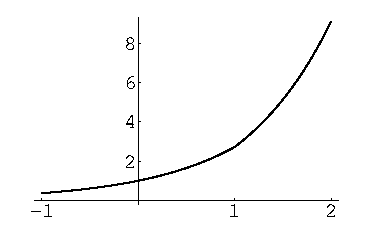
\includegraphics[width=0.4\textwidth]{ode/first_order/heavi}
    \end{center}
    \caption{The solution is continuous.}
    \label{heaviside}
  \end{figure}

\end{Example}
















\begin{Example}
  Consider the problem,
  \[ 
  y' + \sign(x) y = 0, \qquad y(1) = 1.
  \]
  Recall that 
  \[ 
  \sign x = 
  \begin{cases}
    -1 \quad &\mathrm{for}\ x < 0 \\
    0 \quad &\mathrm{for}\ x = 0 \\
    1 \quad &\mathrm{for}\ x > 0. 
  \end{cases}
  \]
  Since $\sign x$ is piecewise defined, we solve the two problems,
  \begin{alignat*}{3}
    y_+' + y_+ &= 0, &\qquad y_+(1) &= 1, &\qquad &\mathrm{for}\ x > 0 \\
    y_-' - y_- &= 0, &\qquad y_-(0) &= y_+(0), &\qquad &\mathrm{for}\ x < 0,
  \end{alignat*}
  and define the solution, $y$, to be
  \[ y(x) = 
  \begin{cases}
    y_+(x), \quad &\mathrm{for}\ x \geq 0, \\
    y_-(x), \quad &\mathrm{for}\ x \leq 0.
  \end{cases} \]
  The initial condition for $y_-$ demands that the solution be continuous.

  Solving the two problems for positive and negative $x$, we obtain
  \[ 
  y(x) = 
  \begin{cases}
    \e^{1-x},       \quad &\mathrm{for}\ x > 0, \\
    \e^{1+x}, \quad &\mathrm{for}\ x < 0.
  \end{cases} 
  \]
  This can be simplified to
  \[ 
  \boxed{
    y(x) = \e^{1 -|x|}.
    }
  \]
  This solution is graphed in Figure~\ref{figure epem}.

  \begin{figure}[tb!]
    \begin{center}
      \includegraphics[width=0.4\textwidth]{ode/first_order/epem}
    \end{center}
    \caption{The solution.} 
    \label{figure epem}
  \end{figure}

\end{Example}





\begin{Result}
  \label{first_order_inhom}
  \textbf{Existence, Uniqueness Theorem.}
  Let $p(x)$ and $f(x)$ be piecewise continuous on the interval $[a,b]$
  and let $x_0 \in [a,b]$.  Consider the problem,
  \[ 
  \frac{\dd y}{\dd x} + p(x) y = f(x), \qquad y(x_0) = y_0.
  \]
  The general solution of the differential equation is
  \[ 
  y = \e^{-P(x)} \int \e^{P(x)}f(x)\,\dd x + c \e^{-P(x)}.
  \]
  The unique, continuous solution of the differential equation 
  subject to the initial condition is
  \[
  y = \e^{-P(x)}\int^x_{x_0} \e^{P(\xi)}f(\xi)\,\dd \xi + y_0 \e^{P(x_0)-P(x)},
  \]
  where $P(x) = \int p(x)\,\dd x$.
\end{Result}









%% \frac{\dd y}{\dd x} + x y = x^{2n+1}, \quad y(1) = 1, \quad n \in \mathbb{Z}
\begin{Exercise}[mathematica/ode/first\_order/exact.nb]
  \label{exercise dydx + x y = x 2n+1}
  Find the solutions of the following differential equations which satisfy the 
  given initial conditions:
  \begin{enumerate}
  \item
    $ \displaystyle
    \frac{\dd y}{\dd x} + x y = x^{2n+1}, \quad y(1) = 1, \quad n \in \mathbb{Z}
    $
  \item
    $ \displaystyle
    \frac{\dd y}{\dd x} - 2 x y = 1, \quad y(0) = 1
    $
  \end{enumerate}

  \hintsolution{dydx + x y = x 2n+1}
\end{Exercise}






%% \frac{\dd y}{\dd x} + \alpha y(x) = \beta \e^{-\lambda x}
\begin{Exercise}[mathematica/ode/first\_order/exact.nb]
  \label{exercise dydx + alpha y = beta e}
  Show that if $\alpha > 0$ and $\lambda > 0$, then for any real $\beta$, 
  every solution of 
  \[
  \frac{\dd y}{\dd x} + \alpha y(x) = \beta \e^{-\lambda x}
  \]
  satisfies $\lim_{x \to +\infty} y(x) = 0$.  (The case $\alpha = \lambda$
  requires special treatment.)  Find the solution for $\beta = \lambda = 1$
  which satisfies $y(0) = 1$.  Sketch this solution for $0 \leq x < \infty$
  for several values of $\alpha$.  In particular, show what happens when
  $\alpha \to 0$ and $\alpha \to \infty$.

  \hintsolution{dydx + alpha y = beta e}
\end{Exercise}










%%===========================================================================
\section{Well-Posed Problems}
\index{well-posed problems}
\index{ill-posed problems}





\begin{Example}
  Consider the problem,
  \[ 
  y' - \frac{1}{x} y = 0, \qquad y(0) = 1.
  \]
  The general solution is $y = c x$.  Applying the initial condition demands that
  $1 = c \cdot 0$, which cannot be satisfied.
  The general solution for various values of $c$ is plotted in 
  Figure~\ref{cx}.

  \begin{figure}[tb!]
    \begin{center}
      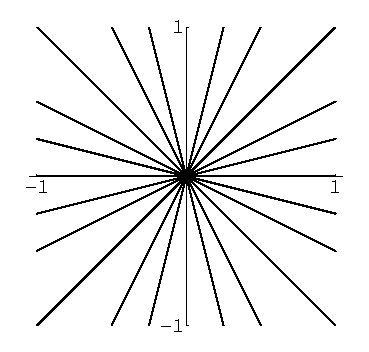
\includegraphics[width=0.3\textwidth]{ode/first_order/cx}
    \end{center}
    \caption{The general solution for various values of the constant
    of integration.}
    \label{cx}
  \end{figure}

\end{Example}








\begin{Example}
  Consider the problem
  \[ 
  y' - \frac{1}{x} y = -\frac{1}{x}, \qquad y(0) = 1.
  \]
  The general solution is 
  \[ 
  y = 1 + c x.
  \]
  The initial condition is satisfied for any value of $c$ so there are an 
  infinite number of solutions.
\end{Example}






\begin{Example}
  Consider the problem
  \[ 
  y' + \frac{1}{x} y = 0, \qquad y(0) = 1.
  \]
  The general solution is $y = \frac{c}{x}$.  
  Depending on whether $c$ is nonzero, the solution is either singular or zero 
  at the origin and cannot satisfy the initial condition.
\end{Example}




The above problems in which there were either no solutions or an infinite
number of solutions are said to be \textit{ill-posed}.  
If there is a unique solution that satisfies the initial condition, 
the problem is said to be \textit{well-posed}.  We should have suspected that
we would run into trouble in the above examples as the initial condition 
was given at a singularity of the coefficient function, $p(x) = 1/x$.

Consider the problem,
\[
y' + p(x) y = f(x), \qquad y(x_0) = y_0.
\]
We assume that $f(x)$ bounded in a neighborhood of $x = x_0$.
The differential equation has the general solution,
\[ 
y = \e^{-P(x)} \int \e^{P(x)}f(x)\,\dd x + c \e^{-P(x)}.
\]
If the homogeneous solution, $\e^{-P(x)}$, is nonzero and finite at $x = x_0$, 
then there is a unique value of $c$ for which the initial condition is 
satisfied.   If the homogeneous solution vanishes at $x = x_0$ then either
the initial condition cannot be satisfied or the initial condition is
satisfied for all values of $c$.   The homogeneous solution can vanish
or be infinite only if $P(x) \to \pm \infty$ as $x \to x_0$.   This can
occur only if the coefficient function, $p(x)$, is unbounded at that point.













\begin{Result}
  If the initial condition is given where the homogeneous solution to a first 
  order, linear differential equation is zero or infinite then the problem 
  may be ill-posed.  This may occur only if the coefficient function,
  $p(x)$, is unbounded at that point.
\end{Result}









%%=============================================================================
\section{Equations in the Complex Plane}
\index{complex plane!first order differential equations}




%%----------------------------------------------------------------------------
\subsection{Ordinary Points}
\index{ordinary points!first order differential equations}




Consider the first order homogeneous equation
\[ 
\frac{\dd w}{\dd z} + p(z) w = 0, 
\]
where $p(z)$, a function of a complex variable, is analytic in some domain $D$.
The integrating factor,
\[ 
I(z) = \exp \left( \int p(z) \,\dd z \right),
\]
is an analytic function in that domain.  As with the case of real variables, 
multiplying by the integrating factor and integrating yields the solution,
\[
w(z) = c \exp\left(-\int p(z)\,\dd z \right). 
\] 
We see that the solution is analytic in $D$. 





\begin{Example} 
  It does not make sense to pose the equation
  \[ \frac{\dd w}{\dd z} + |z| w = 0. \]
  For the solution to exist, $w$ and hence $w'(z)$ must be analytic.  
  Since $p(z) = |z|$ is not analytic anywhere in the complex plane, the
  equation has no solution.
\end{Example}




Any point at which $p(z)$ is analytic is called an \textit{ordinary point} 
of the differential equation.
Since the solution is analytic we can expand it in a Taylor series about
an ordinary point. The radius of convergence of the series will be at least the 
distance to the nearest singularity of $p(z)$ in the complex plane.




\begin{Example} 
  \label{ssrp_expand_solution}
  Consider the equation
  \[ 
  \frac{\dd w}{\dd z} - \frac{1}{1-z} w = 0.
  \]
  The general solution is $w = \frac{c}{1-z}.$  Expanding this solution 
  about the origin,
  \[ 
  w = \frac{c}{1-z} = c\sum_{n=0}^\infty z^n.
  \]
  The radius of convergence of the series is,
  \[
  R = \lim_{n \to \infty} \left|\frac{a_n}{a_{n+1}} \right| = 1,
  \]
  which is the distance from the origin to the nearest singularity of 
  $p(z) = \frac{1}{1-z}$.
\end{Example}




We do not need to solve the differential equation to find the Taylor series
expansion of the homogeneous solution.  
\index{Taylor series!first order differential equations}
We could substitute a general Taylor series expansion into
the differential equation and solve for the coefficients.  Since we can 
always solve first order equations, this method is of limited usefulness.
However, when we consider higher order equations in which we cannot 
solve the equations exactly, this will become an important method.




\begin{Example}
  Again consider the equation
  \[ 
  \frac{\dd w}{\dd z} - \frac{1}{1-z} w = 0.
  \]
  Since we know that the solution has a Taylor series expansion about $z=0$,
  we substitute $w = \sum_{n=0}^\infty a_n z^n$ into the differential equation.
  \begin{gather*}
    (1-z) \frac{\dd}{\dd z} \sum_{n=0}^\infty a_n z^n 
    - \sum_{n=0}^\infty a_n z^n = 0 \\
    \sum_{n=1}^\infty n a_n z^{n-1} - \sum_{n=1}^\infty n a_n z^n 
    - \sum_{n=0}^\infty a_n z^n = 0 \\
    \sum_{n=0}^\infty (n+1) a_{n+1} z^n - \sum_{n=0}^\infty n a_n z^n 
    - \sum_{n=0}^\infty a_n z^n = 0 \\
    \sum_{n=0}^\infty \left((n+1) a_{n+1} - (n+1) a_n \right) z^n = 0.
  \end{gather*}
  Now we equate powers of $z$ to zero.  For $z^n$, the equation is 
  $(n+1) a_{n+1} - (n+1) a_n = 0$, or $a_{n+1} = a_n$.  Thus we have that
  $a_n = a_0$ for all $n \geq 1$.  The solution is then
  \[ 
  \boxed{ 
    w = a_0 \sum_{n=0}^\infty z^n, 
    } 
  \]
  which is the result we obtained by expanding the solution in 
  Example~\ref{ssrp_expand_solution}.
\end{Example}




\begin{Result}
  Consider the equation
  \[ 
  \frac{\dd w}{\dd z} + p(z) w = 0. 
  \]
  If $p(z)$ is analytic at $z = z_0$ then $z_0$ is called an ordinary point
  of the differential equation.  The Taylor series expansion of the solution
  can be found by substituting $w = \sum_{n=0}^\infty a_n (z-z_0)^n$ into the 
  equation and equating powers of $(z-z_0)$.  The radius of convergence of the
  series is at least the distance to the nearest singularity of $p(z)$ in 
  the complex plane.
\end{Result}






%% Taylor series about origin
\begin{Exercise} 
  \label{exercise dwdz + 1 1-z w}
  Find the Taylor series expansion about the origin of the solution to
  \[
  \frac{\dd w}{\dd z} + \frac{1}{1-z} w = 0
  \]
  with the substitution $w = \sum_{n=0}^\infty a_n z^n$.  What is the 
  radius of convergence of the series?  What is the distance to the nearest
  singularity of $\frac{1}{1-z}$?

  \hintsolution{dwdz + 1 1-z w}
\end{Exercise}











%%----------------------------------------------------------------------------
\subsection{Regular Singular Points}
\index{regular singular points!first order differential equations}



If the coefficient function $p(z)$ has a simple pole at $z = z_0$ then $z_0$ 
is a \textit{regular singular point} of the first order differential equation.





\begin{Example}
  Consider the equation
  \[
  \frac{\dd w}{\dd z} + \frac{\alpha}{z} w = 0, \qquad \alpha \neq 0.
  \]
  This equation has a regular singular point at $z = 0$.
  The solution is $w = c z^{-\alpha}$.  Depending on the value of $\alpha$, the
  solution can have three different kinds of behavior.

  \begin{description}
    %%
  \item{$\boldsymbol{\alpha}$ \textbf{is a negative integer.}}
    The solution is analytic in the finite complex plane.
    %%
  \item{$\boldsymbol{\alpha}$ \textbf{is a positive integer}}
    The solution has a pole at the origin.  
    $w$ is analytic in the annulus, $0<|z|$.
    %%
  \item{$\boldsymbol{\alpha}$ \textbf{is not an integer.}}
    $w$ has a branch point at $z=0$.
    The solution is analytic in the cut annulus $0 < |z| < \infty $, 
    $\theta_0 < \arg z < \theta_0 + 2 \pi$.
  \end{description}
\end{Example}




Consider the differential equation
\[ 
\frac{\dd w}{\dd z} + p(z) w = 0, 
\]
where $p(z)$ has a simple pole at the origin and is analytic in the annulus, 
$0 < |z| < r$, for some positive $r$.  Recall that the solution is
\begin{align*}
  w       &= c \exp \left(- \int p(z)\,\dd z \right) \\
  &= c \exp \left(- \int \frac{b_0}{z} + p(z) - \frac{b_0}{z} \,\dd z 
  \right) \\
  &= c \exp \left( - b_0 \log z - \int \frac{z p(z) - b_0}{z} \,\dd z 
  \right) \\
  &= c z^{-b_0} \exp \left(  - \int \frac{z p(z) - b_0}{z} \,\dd z \right)
\end{align*}

The exponential factor has a removable singularity at $z = 0$ and is analytic 
in $|z| < r$.  We consider the following cases for the $z^{-b_0}$ factor:
\begin{description}
  %%
\item{$\mathbf{b_0}$ \textbf{is a negative integer.}}
  Since $z^{-b_0}$ is analytic at the origin, the solution to the differential
  equation is analytic in the circle $|z| < r$.
  %%
\item{$\mathbf{b_0}$ \textbf{is a positive integer.}}
  The solution has a pole of order $-b_0$ at the origin and is analytic
  in the annulus $0 < |z| < r$.
  %%
\item{$\mathbf{b_0}$ \textbf{is not an integer.}}
  The solution has a branch point at the origin and thus is not single-valued.
  The solution is analytic in the cut annulus $0 < |z| < r$, 
  $\theta_0 < \arg z < \theta_0 + 2\pi$.
\end{description}

Since the exponential factor has a convergent Taylor series in $|z|<r$,
the solution can be expanded in a series of the form
\index{Laurent series!first order differential equation}
\[ 
w = z^{-b_0} \sum_{n=0}^\infty a_n z^n, 
\quad \mathrm{where}\ a_0 \neq 0\ 
\mathrm{and}\ b_0 = \lim_{z \to 0} z\,p(z).
\]
In the case of a regular singular point at $z = z_0$, the series is
\[ 
w = (z - z_0)^{-b_0} \sum_{n=0}^\infty a_n (z-z_0)^n, 
\quad \mathrm{where}\ a_0 \neq 0\ 
\mathrm{and}\ b_0 = \lim_{z \to z_0}(z-z_0)\,p(z).
\]


Series of this form are known as \textit{Frobenius series}. 
\index{Frobenius series!first order differential equation}
Since we can write the solution as
\[ 
w = c (z-z_0)^{-b_0} \exp \left(- \int 
  \left( p(z) - \frac{b_0}{z-z_0} \right) \,\dd z \right),
\]
we see that the Frobenius expansion of the solution will have a radius of 
convergence at least the distance to the nearest singularity of $p(z)$.




\begin{Result}
  Consider the equation,
  \[ 
  \frac{\dd w}{\dd z} + p(z) w = 0,
  \]
  where $p(z)$ has a simple pole at $z=z_0$, $p(z)$ is analytic in some
  annulus, $0 < |z-z_0| < r$, and $\lim_{z \to z_0} (z-z_0) p(z) = \beta$.
  The solution to the differential equation has a Frobenius series expansion
  of the form
  \[ 
  w = (z-z_0)^{-\beta} \sum_{n=0}^\infty a_n (z-z_0)^n, \qquad a_0 \neq 0.
  \]
  The radius of convergence of the expansion will be at least the 
  distance to the nearest singularity of $p(z)$.
\end{Result}








\begin{Example}
  We will find the first two nonzero terms in the series solution about $z = 0$ 
  of the differential equation,
  \[ 
  \frac{\dd w}{\dd z} + \frac{1}{\sin z} w = 0.
  \]
  First we note that the coefficient function has a simple pole at $z = 0$ and
  \[ 
  \lim_{z \to 0} \frac{z}{\sin z} = \lim_{z \to 0} \frac{1}{\cos z} = 1.
  \]
  Thus we look for a series solution of the form
  \[ 
  w = z^{-1} \sum_{n=0}^\infty a_n z^n, \qquad a_0 \neq 0.
  \]
  The nearest singularities of $1 / \sin z$ in the complex plane are at 
  $z = \pm \pi$.  Thus the radius of convergence of the series will
  be at least $\pi$.

  Substituting the first three terms of the expansion into the differential 
  equation,
  \begin{gather*}
    \frac{\dd}{\dd z}(a_0 z^{-1} + a_1 + a_2 z) 
    + \frac{1}{\sin z} (a_0 z^{-1} + a_1 + a_2 z) = O(z). \\
    \intertext{Recall that the Taylor expansion of $\sin z$ is 
      $\sin z = z - \frac{1}{6}z^3 + O(z^5)$.}
    \left(z - \frac{z^3}{6} + O(z^5)\right)
    (-a_0 z^{-2} + a_2) + (a_0 z^{-1} + a_1 + a_2 z) = O(z^2)\\
    -a_0 z^{-1} + \left(a_2 + \frac{a_0}{6}\right)z + a_0 z^{-1} + a_1 + a_2 z 
    = O(z^2) \\
    a_1 + \left(2a_2 + \frac{a_0}{6}\right) z = O(z^2)
  \end{gather*}
  $a_0$ is arbitrary.  Equating powers of $z$,
  \begin{align*}
    &z^0: \qquad a_1 = 0. \\
    &z^1: \qquad 2a_2 + \frac{a_0}{6} = 0.
  \end{align*}
  Thus the solution has the expansion,
  \[
  \boxed{
    w = a_0 \left(z^{-1} - \frac{z}{12} \right) + O(z^2).
    }
  \]
  In Figure~\ref{figure foode oosc} the exact solution is plotted in a solid 
  line and the two term approximation is plotted in a dashed line.  The two
  term approximation is very good near the point $x = 0$.

  \begin{figure}[tb!]
    \begin{center}
      \includegraphics[width=0.4\textwidth]{ode/first_order/oosc}
    \end{center}
    \caption{Plot of the exact solution and the two term approximation.}
    \label{figure foode oosc}
  \end{figure}

\end{Example}














\begin{Example}
  Find the first two nonzero terms in the series expansion about $z=0$ 
  of the solution to
  \[
  w' - i \frac{\cos z}{z} w = 0.
  \]
  Since $\frac{\cos z}{z}$ has a simple pole at $z=0$ and 
  $\lim_{z \to 0} -i \cos z = -i$
  we see that the Frobenius series will have the form
  \[ 
  w = z^i \sum_{n=0}^\infty a_n z^n, \qquad a_0 \neq 0.
  \]
  Recall that $\cos z$ has the Taylor expansion 
  $\sum_{n=0}^\infty \frac{(-1)^n z^{2n}}{(2n)!}$.  
  Substituting the Frobenius expansion into the differential equation yields
  \begin{gather*}
    z \left( i z^{i-1} \sum_{n=0}^\infty a_n z^n 
      + z^i \sum_{n=0}^\infty n a_n z^{n-1} \right)
    - i \left(\sum_{n=0}^\infty \frac{(-1)^n z^{2n}}{(2n)!}\right)
    \left( z^i \sum_{n=0}^\infty a_n z^n\right) = 0 \\
    \sum_{n=0}^\infty(n+i)a_n z^n 
    -i  \left(\sum_{n=0}^\infty \frac{(-1)^n z^{2n}}{(2n)!}\right)
    \left(\sum_{n=0}^\infty a_n z^n\right) = 0. 
  \end{gather*}
  Equating powers of $z$,
  \begin{alignat*}{2}
    &z^0:   &\quad  &i a_0 -i a_0 = 0 \qquad \to a_0\ \mathrm{is arbitrary} \\
    &z^1:   &\quad  &(1+i)a_1 - i a_1 = 0 \qquad \to a_1 = 0 \\
    &z^2:   &\quad  &(2+i)a_2 - i a_2 + \frac{i}{2} a_0 = 0 
    \qquad \to a_2 = -\frac{i}{4}a_0.
  \end{alignat*}
  Thus the solution is
  \[ 
  \boxed{
    w = a_0 z^i \left(1 -\frac{i}{4}z^2 + O(z^3) \right).
    }
  \]
\end{Example}











%%----------------------------------------------------------------------------
\subsection{Irregular Singular Points}
\index{irregular singular points!first order differential equations}


If a point is not an ordinary point or a regular singular point then it 
is called an \textit{irregular singular point}. The following equations have
irregular singular points at the origin.
\begin{itemize}
\item $w' + \sqrt{z} w = 0$ 
\item $w' - z^{-2} w = 0$ 
\item $w' + \exp(1/z) w = 0$
\end{itemize}





\begin{Example}
  Consider the differential equation
  \[ 
  \frac{\dd w}{\dd z}  + \alpha z^\beta w = 0, 
  \qquad \alpha \neq 0, \quad \beta \neq -1, 0, 1, 2, \ldots
  \]
  This equation has an irregular singular point at the origin.
  Solving this equation,
  \begin{gather*}
    \frac{\dd}{\dd z} \left(\exp\left(\int \alpha z^\beta\,\dd z \right) w \right)=0\\
    \boxed{ 
      w = c \exp \left(- \frac{\alpha}{\beta+1} z^{\beta+1}\right) = 
      c \sum_{n = 0}^\infty \frac{(-1)^n}{n!} \left( \frac{\alpha}{\beta+1} \right)^n
      z^{(\beta+1)n}. 
      }
  \end{gather*}
  If $\beta$ is not an integer, then the solution has a branch point at the
  origin.  If $\beta$ is an integer, $\beta < -1$, then the solution
  has an essential singularity at the origin.
  The solution cannot be expanded in a Frobenius series,
  $w = z^\lambda \sum_{n=0}^\infty a_n z^n$.  
\end{Example}




Although we will not show it, this result holds for any irregular singular
point of the differential equation.  We cannot approximate 
the solution near an irregular singular point using a Frobenius expansion.

Now would be a good time to summarize what we have discovered about
solutions of first order differential equations in the complex plane.


\begin{Result}
  Consider the first order differential equation
  \[ 
  \frac{\dd w}{\dd z} + p(z) w = 0.
  \]
  \begin{description}
    %%
  \item{\textbf{Ordinary Points}}  If $p(z)$ is analytic at $z=z_0$ then
    $z_0$ is an ordinary point of the differential equation.  The solution can be 
    expanded in the Taylor series $w = \sum_{n=0}^\infty a_n (z-z_0)^n$.  The
    radius of convergence of the series is at least the distance to the nearest
    singularity of $p(z)$ in the complex plane.
    %%
  \item{\textbf{Regular Singular Points}} If $p(z)$ has a simple pole at 
    $z = z_0$ and is analytic in some annulus $0 < |z-z_0| < r$ then $z_0$
    is a regular singular point of the differential equation.  The solution
    at $z_0$ will either be analytic, have a pole, or have a branch point.
    The solution can be expanded in the Frobenius series
    $w = (z-z_0)^{-\beta} \sum_{n=0}^\infty a_n (z-z_0)^n$ where $a_0 \neq 0$
    and $\beta = \lim_{z \to z_0} (z-z_0) p(z)$.  The radius of convergence of the
    Frobenius series will be at least the distance to the nearest singularity
    of $p(z)$.
    %%
  \item{\textbf{Irregular Singular Points}} If the point $z=z_0$ is not
    an ordinary point or a regular singular point, then it is an irregular singular
    point of the differential equation.  The solution cannot be expanded in a 
    Frobenius series about that point.
  \end{description}
\end{Result}








%%----------------------------------------------------------------------------
\subsection{The Point at Infinity}
\label{fode:section:ecp:sub:pi}
\index{infinity!first order differential equation}


Now we consider the behavior of first order linear differential equations
at the point at infinity.  Recall from complex variables that the 
complex plane together with the point at infinity is called the
extended complex plane.  To study the behavior of a function $f(z)$ at 
infinity, we make the transformation $z = \frac{1}{\zeta}$ and study the 
behavior of $f(1/\zeta)$ at $\zeta=0$.


\begin{Example}
  Let's examine the behavior of $\sin z$ at infinity.  We make the substitution
  $z = 1/\zeta$ and find the Laurent expansion about $\zeta=0$.
  \[
  \sin(1/\zeta) = \sum_{n=0}^\infty \frac{(-1)^n}{(2n+1)! \, \zeta^{(2n+1)}}
  \]
  Since $\sin(1/\zeta)$ has an essential singularity at $\zeta=0$,
  $\sin z$ has an essential singularity at infinity.
\end{Example}




We use the same approach if we want to examine the behavior at infinity of a 
differential equation.  Starting with the first order differential equation,
\[ 
\frac{\dd w}{\dd z} + p(z) w = 0,
\]
we make the substitution
\[ 
z = \frac{1}{\zeta}, \qquad \frac{\dd}{\dd z} = -\zeta^2 \frac{\dd}{\dd \zeta}, 
\qquad w(z) = u(\zeta) 
\]
to obtain
\begin{gather*}
  -\zeta^2 \frac{\dd u}{\dd \zeta} + p(1/\zeta) u = 0 \\
  \frac{\dd u}{\dd \zeta} - \frac{p(1/\zeta)}{\zeta^2} u = 0.
\end{gather*}




\begin{Result}
  The behavior at infinity of
  \[ 
  \frac{\dd w}{\dd z} + p(z) w = 0
  \]
  is the same as the behavior at $\zeta=0$ of
  \[
  \frac{\dd u}{\dd \zeta} - \frac{p(1/\zeta)}{\zeta^2} u = 0.
  \]
\end{Result}






\begin{Example}
  We classify the singular points of the equation
  \[
  \frac{\dd w}{\dd z} + \frac{1}{z^2 + 9} w = 0.
  \]
  We factor the denominator of the fraction 
  to see that $z = \imath 3$ and $z = - \imath 3$ are regular singular points.  
  \[
  \frac{\dd w}{\dd z} + \frac{1}{(z - \imath 3)(z + \imath 3)} w = 0
  \]
  We make the transformation $z = 1 / \zeta$ to examine the point at infinity.
  \begin{gather*}
    \frac{\dd u}{\dd \zeta} - \frac{1}{\zeta^2}\frac{1}{(1/\zeta)^2+9} u = 0 
    \\
    \frac{\dd u}{\dd \zeta} - \frac{1}{9 \zeta^2 + 1} u = 0 
  \end{gather*}
  Since the equation for $u$ has a ordinary point at $\zeta = 0$, 
  $z = \infty$ is a ordinary point of the equation for $w$.
\end{Example}






















\raggedbottom
%%============================================================================
\exercises{
\pagebreak
\flushbottom
\section{Additional Exercises}





%%-----------------------------------------------------------------------------
\begin{large}
  \noindent
  \textbf{Exact Equations}
\end{large}





\begin{Exercise}[mathematica/ode/first\_order/exact.nb]
  \label{exercise dydx=xxyyx}
  Find the general solution $y=y(x)$ of the equations
  \begin{enumerate}
    \centering
  \item
    $\displaystyle \frac{\dd y}{\dd x} = \frac{ x^2 + x y + y^2 }{ x^2 }$,
  \item
    $\displaystyle (4y-3x) \,\dd x + (y-2x) \,\dd y = 0$.
  \end{enumerate}

  \hintsolution{dydx=xxyyx}
\end{Exercise}









\begin{Exercise}[mathematica/ode/first\_order/exact.nb]
  \label{exercise dydx=axbybxcy}
  Determine whether or not the following equations can be made exact.
  If so find the corresponding general solution.
  \begin{enumerate}
    \centering
  \item
    $\displaystyle (3x^2-2xy+2) \,\dd x+(6y^2-x^2+3) \,\dd y = 0$
  \item
    $\displaystyle \frac{\dd y}{\dd x}=-\frac{ax+by}{bx+cy}$
  \end{enumerate}

  \hintsolution{dydx=axbybxcy}
\end{Exercise}





\begin{Exercise}[mathematica/ode/first\_order/exact.nb]
  \label{exercise dydx = 1-2x y2}
  Find the solutions of the following differential equations
  which satisfy the given initial condition. In each case determine
  the interval in which the solution is defined.
  \begin{enumerate}
    \centering
  \item
    $\displaystyle \frac{\dd y}{\dd x} = (1-2x) y^2, \quad y(0) = -1/6$.
  \item
    $\displaystyle x \,\dd x + y \e^{-x} \,\dd y = 0, \quad y(0) = 1$.
  \end{enumerate}

  \hintsolution{dydx = 1-2x y2}
\end{Exercise}








%% (4 y - x) y' - (9 x^2 + y - 1) = 0.
\begin{Exercise}
  \label{exercise 4yxy9x2y10}
  Are the following equations exact?  If so, solve them.
  \begin{enumerate}
  \item
    $ \displaystyle
    (4 y - x) y' - (9 x^2 + y - 1) = 0
    $
  \item
    $ \displaystyle
    (2 x - 2 y) y' + (2 x + 4 y) = 0.
    $
  \end{enumerate}

  \hintsolution{4yxy9x2y10}
\end{Exercise}










%% y^2 \sin t + y f(t) \frac{\dd y}{\dd t} = 0
\begin{Exercise}[mathematica/ode/first\_order/exact.nb]
  \label{exercise y2 sin t + y f dydt}
  Find all functions $f(t)$ such that the differential equation
  \begin{equation}
    \label{eqn_y2_sint}
    y^2 \sin t + y f(t) \frac{\dd y}{\dd t} = 0
  \end{equation}
  is exact.  Solve the differential equation for these $f(t)$.

  \hintsolution{y2 sin t + y f dydt}
\end{Exercise}






%%-----------------------------------------------------------------------------
\begin{large}
  \noindent
  \textbf{The First Order, Linear Differential Equation}
\end{large}



%% y' + \frac{y}{\sin x} = 0. 
\begin{Exercise}[mathematica/ode/first\_order/linear.nb]
  \label{exercise y + y / sin x}
  Solve the differential equation
  \[ 
  y' + \frac{y}{\sin x} = 0. 
  \]

  \hintsolution{y + y / sin x}
\end{Exercise}




%%-----------------------------------------------------------------------------
\begin{large}
  \noindent
  \textbf{Initial Conditions}
\end{large}







%%-----------------------------------------------------------------------------
\begin{large}
  \noindent
  \textbf{Well-Posed Problems}
\end{large}





%% t \frac{\dd y}{\dd t} + A y = 1 + t^2
\begin{Exercise}
  \label{exercise t dydt + A y}
  Find the solutions of
  \[
  t \frac{\dd y}{\dd t} + A y = 1 + t^2, \quad t > 0
  \]
  which are bounded at $t = 0$.  Consider all (real) values of $A$.

  \hintsolution{t dydt + A y}
\end{Exercise}



%%-----------------------------------------------------------------------------
\begin{large}
  \noindent
  \textbf{Equations in the Complex Plane}
\end{large}




%% Classify the singular points of the following first order differential
\begin{Exercise} 
  \label{exercise dwdz + sin z z w}
  Classify the singular points of the following first order differential
  equations, (include the point at infinity).
  \begin{enumerate}
  \item $w' + \frac{\sin z}{z} w = 0$
  \item $w' + \frac{1}{z-3} w = 0$
  \item $w' + z^{1/2} w = 0$
  \end{enumerate}

  \hintsolution{dwdz + sin z z w}
\end{Exercise}







%% Expand irregular singular point in a Frobenius series.
\begin{Exercise} 
  \label{exercise dwdz z-2 w}
  Consider the equation
  \[ 
  w' + z^{-2}w = 0.
  \]
  The point $z = 0$ is an irregular singular point of the differential
  equation.  Thus we know that we cannot expand the solution about
  $z=0$ in a Frobenius series.  Try substituting the series solution
  \[
  w = z^\lambda \sum_{n=0}^\infty a_n z^n, \qquad a_0 \neq 0
  \]
  into the differential equation anyway.  What happens?

  \hintsolution{dwdz z-2 w}
\end{Exercise}



































\raggedbottom
}
%%============================================================================
\pagebreak
\flushbottom
\section{Hints}



%% Solve first order equations by inspection.
\begin{Hint}
  \label{hint gygyf}
  $\phantom{a}$

  \begin{enumerate}
    %%
  \item $\frac{\dd}{\dd x} \ln |u| = \frac{1}{u}$
    %%
  \item $\frac{\dd}{\dd x} u^c = u^{c-1} u'$
  \end{enumerate}
\end{Hint}






%% \mu(x,y) = \frac{1}{x M(x,y) + y N(x,y)}
\begin{Hint}
  \label{hint integrating factor homogeneous}
  %% CONTINUE
\end{Hint}





%% $d y / d t = f(y / t)$.
\begin{Hint}
  \label{hint dydt = f(y/t)}
  The equation is homogeneous.  Make the change of variables $u = y / t$.
\end{Hint}




%% y' - \frac{1}{x} y = x^\alpha.
\begin{Hint}
  \label{hint y - 1/x y = x alpha}
  Make sure you consider the case $\alpha = 0$.
\end{Hint}




%% \frac{\dd y}{\dd x} + x y = x^{2n+1}, \quad y(1) = 1, \quad n \in \mathbb{Z}
\begin{Hint}
  \label{hint dydx + x y = x 2n+1}
  %% CONTINUE
\end{Hint}



%% \frac{\dd y}{\dd x} + \alpha y(x) = \beta \e^{-\lambda x}
\begin{Hint}
  \label{hint dydx + alpha y = beta e}
  %% CONTINUE
\end{Hint}





%% Taylor series about origin
\begin{Hint} 
  \label{hint dwdz + 1 1-z w}
  The radius of convergence of the series and the distance to the nearest 
  singularity of $\frac{1}{1-z}$ are not the same.
\end{Hint}








\hints{
%%-----------------------------------------------------------------------------
\begin{large}
  \noindent
  \textbf{Exact Equations}
\end{large}



\begin{Hint}
  \label{hint dydx=xxyyx}
  \begin{enumerate}
  \item
  \item
  \end{enumerate}
\end{Hint}




\begin{Hint}
  \label{hint dydx=axbybxcy}
  \begin{enumerate}
  \item
    The equation is exact.  Determine the primitive $u$ by solving the equations
    $u_x = P$, $u_y = Q$.
  \item
    The equation can be made exact.
  \end{enumerate}
\end{Hint}






\begin{Hint}
  \label{hint dydx = 1-2x y2}
  \begin{enumerate}
  \item
    This equation is separable.  Integrate to get the general solution.
    Apply the initial condition to determine the constant of integration.
  \item
    Ditto.  You will have to numerically solve an equation to determine where
    the solution is defined.
  \end{enumerate}
\end{Hint}






%% (4 y - x) y' - (9 x^2 + y - 1) = 0.
\begin{Hint}
  \label{hint 4yxy9x2y10}
  %% CONTINUE
\end{Hint}










%% y^2 \sin t + y f(t) \frac{\dd y}{\dd t} = 0
\begin{Hint}
  \label{hint y2 sin t + y f dydt}
  %% CONTINUE
\end{Hint}





%%-----------------------------------------------------------------------------
\begin{large}
  \noindent
  \textbf{The First Order, Linear Differential Equation}
\end{large}



%% y' + \frac{y}{\sin x} = 0. 
\begin{Hint}
  \label{hint y + y / sin x}
  Look in the appendix for the integral of $\csc x$.
\end{Hint}




%%-----------------------------------------------------------------------------
\begin{large}
  \noindent
  \textbf{Initial Conditions}
\end{large}





%%-----------------------------------------------------------------------------
\begin{large}
  \noindent
  \textbf{Well-Posed Problems}
\end{large}




%% t \frac{\dd y}{\dd t} + A y = 1 + t^2
\begin{Hint}
  \label{hint t dydt + A y}
  %% CONTINUE
\end{Hint}







%%-----------------------------------------------------------------------------
\begin{large}
  \noindent
  \textbf{Equations in the Complex Plane}
\end{large}



%% Classify the singular points of the following first order differential
\begin{Hint}
  \label{hint dwdz + sin z z w}
  %% CONTINUE
\end{Hint}



%% Expand irregular singular point in a Frobenius series.
\begin{Hint}
  \label{hint dwdz z-2 w}
  Try to find the value of $\lambda$ by substituting the series into the 
  differential equation and equating powers of $z$.
\end{Hint}


















\raggedbottom
}
%%============================================================================
\pagebreak
\flushbottom
\section{Solutions}



%% Solve first order equations by inspection.
\begin{Solution}
  \label{solution gygyf}
  $\phantom{a}$

  \begin{enumerate}
    %%
  \item
    \begin{gather*}
      \frac{y'(x)}{y(x)} = f(x) 
      \\
      \frac{\dd}{\dd x} \ln |y(x)| = f(x) 
      \\
      \ln |y(x)| = \int f(x) \,\dd x + c 
      \\
      y(x) = \pm \e^{\int f(x) \,\dd x + c} 
      \\
      \boxed{
        y(x) = c \e^{\int f(x) \,\dd x} 
        }
    \end{gather*}
    %%
  \item
    \begin{gather*}
      y^\alpha(x) y'(x) = f(x) 
      \\
      \frac{ y^{\alpha+1}(x) }{ \alpha + 1 } = \int f(x)\,\dd x + c 
      \\
      \boxed{
        y(x) = \left( (\alpha+1) \int f(x)\,\dd x + a \right)^{1/(\alpha+1)}
        }
    \end{gather*}
    %%
  \item
    \begin{gather*} 
      \frac{y'}{\cos x} + y \frac{\tan x}{\cos x} = \cos x 
      \\
      \frac{\dd}{\dd x} \left( \frac{y}{\cos x} \right) = \cos x 
      \\
      \frac{y}{\cos x} =  \sin x + c 
      \\
      \boxed{ 
        y(x) = \sin x \cos x + c \cos x
        } 
    \end{gather*}
  \end{enumerate}
\end{Solution}





%% \mu(x,y) = \frac{1}{x M(x,y) + y N(x,y)}
\begin{Solution}
  \label{solution integrating factor homogeneous}
  We consider the homogeneous equation,
  \[
  P(x,y) + Q(x,y) \frac{\dd y}{\dd x} = 0.
  \]
  That is, both $P$ and $Q$ are homogeneous of degree $n$.  We hypothesize 
  that multiplying by
  \[
  \mu(x,y) = \frac{1}{x P(x,y) + y Q(x,y)}
  \]
  will make the equation exact.  To prove this we use the result that 
  \[
  M(x,y) + N(x,y) \frac{\dd y}{\dd x} = 0
  \]
  is exact if and only if $M_y = N_x$.
  \begin{align*}
    M_y &= \frac{\partial}{\partial y} \left[ \frac{ P }{ x P + y Q } \right] 
    \\
    &= \frac{ P_y (x P + y Q) - P (x P_y + Q + y Q_y) }{ (x P + y Q)^2 } 
  \end{align*}
  \begin{align*}
    N_x &= \frac{\partial}{\partial x} \left[ \frac{ Q }{ x P + y Q } \right] 
    \\
    &= \frac{ Q_x (x P + y Q) - Q (P + x P_x + y Q_x) }{ (x P + y Q)^2 }
  \end{align*}
  \begin{gather*}
    M_y = N_x
    \\
    P_y (x P + y Q) - P (x P_y + Q + y Q_y)
    = Q_x (x P + y Q) - Q (P + x P_x + y Q_x) 
    \\
    y P_y Q - y P Q_y = x P Q_x - x P_x Q  
    \\
    x P_x Q + y P_y Q = x P Q_x + y P Q_y 
    \\
    (x P_x + y P_y) Q = P (x Q_x + y Q_y)
    \\
    \intertext{With Euler's theorem, this reduces to an identity.}
    n P Q = P n Q
  \end{gather*}
  Thus the equation is exact.  $\mu(x,y)$ is an integrating factor for 
  the homogeneous equation.
\end{Solution}







%% $d y / d t = f(y / t)$.
\begin{Solution}
  \label{solution dydt = f(y/t)}
  We note that this is a homogeneous differential equation.  The coefficient
  of $\dd y / \dd t$ and the inhomogeneity are homogeneous of degree zero.
  \[
  \frac{\dd y}{\dd t} 
  = 2 \left( \frac{y}{t} \right) + \left( \frac{y}{t} \right)^2.
  \]
  We make the change of variables $u = y / t$ to obtain a separable equation.
  \begin{gather*}
    t u' + u = 2 u + u^2
    \\
    \frac{u'}{u^2 + u} = \frac{1}{t}
  \end{gather*}
  Now we integrate to solve for $u$.
  \begin{gather*}
    \frac{u'}{u(u + 1)} = \frac{1}{t} 
    \\
    \frac{u'}{u} - \frac{u'}{u + 1} = \frac{1}{t} 
    \\
    \ln |u| - \ln |u + 1| = \ln |t| + c 
    \\
    \ln \left| \frac{u}{u + 1} \right| = \ln |c t| 
    \\
    \frac{u}{u + 1} = \pm c t 
    \\
    \frac{u}{u + 1} = c t 
    \\
    u = \frac{c t}{1 - c t} 
    \\
    u = \frac{t}{c - t} 
    \\
    \boxed{
      y = \frac{t^2}{c - t}
      }
  \end{gather*}
\end{Solution}






%% y' - \frac{1}{x} y = x^\alpha.
\begin{Solution}
  \label{solution y - 1/x y = x alpha}
  We consider
  \[
  y' - \frac{1}{x} y = x^{\alpha}, \quad x > 0.
  \]
  First we find the integrating factor.
  \[
  I(x) = \exp\left( \int -\frac{1}{x} \,\dd x \right)
  = \exp\left( -\ln x \right)
  = \frac{1}{x}.
  \]
  We multiply by the integrating factor and integrate.
  \begin{gather*}
    \frac{1}{x} y' - \frac{1}{x^2} y = x^{\alpha - 1} 
    \\
    \frac{\dd}{\dd x} \left( \frac{1}{x} y \right) = x^{\alpha - 1} 
    \\
    \frac{1}{x} y = \int x^{\alpha - 1} \,\dd x + c 
    \\
    y = x \int x^{\alpha - 1} \,\dd x + c x
    \\
    \boxed{
      y = 
      \begin{cases}
        \frac{x^{\alpha + 1}}{\alpha} + c x \quad &\mathrm{for}\ \alpha \neq 0, 
        \\
        x \ln x + c x \quad &\mathrm{for}\ \alpha = 0.
      \end{cases}
      }
  \end{gather*}
\end{Solution}






%% \frac{\dd y}{\dd x} + x y = x^{2n+1}, \quad y(1) = 1, \quad n \in \mathbb{Z}
\begin{Solution}
  \label{solution dydx + x y = x 2n+1}
  \begin{enumerate}
    %%
    %%
  \item
    \[
    y' + x y = x^{2n+1}, \quad y(1) = 1, \quad n \in \mathbb{Z}
    \]
    We find the integrating factor.
    \[
    I(x) = \e^{\int x \,\dd x} = \e^{x^2 / 2}
    \]
    We multiply by the integrating factor and integrate.  Since the initial 
    condition is given at $x = 1$, we will take the lower bound of integration
    to be that point.
    \begin{gather*}
      \frac{\dd}{\dd x} \left( \e^{x^2 / 2} y \right) = x^{2n+1} \e^{x^2 / 2} 
      \\
      y = \e^{-x^2 / 2} \int_1^x \xi^{2n+1} \e^{\xi^2 / 2} \,\dd \xi + c \e^{-x^2 / 2}
    \end{gather*}
    We choose the constant of integration to satisfy the initial condition.
    \[
    \boxed{
      y = \e^{-x^2 / 2} \int_1^x \xi^{2n+1} \e^{\xi^2 / 2} \,\dd \xi + \e^{(1-x^2) / 2}
      }
    \]
    If $n \geq 0$ then we can use integration by parts to write the integral
    as a sum of terms.  If $n < 0$ we can write the integral in terms of 
    the exponential integral function.  However, the integral form above is
    as nice as any other and we leave the answer in that form.
    %%
    %%
  \item
    \[
    \frac{\dd y}{\dd x} - 2 x y(x) = 1, \quad y(0) = 1.
    \]
    We determine the integrating factor and then integrate the equation.
    \begin{gather*}
      I(x) = \e^{\int - 2 x \,\dd x} = \e^{- x^2}
      \\
      \frac{\dd}{\dd x} \left( \e^{-x^2} y \right) = \e^{-x^2} 
      \\
      y = \e^{x^2} \int_0^x \e^{-\xi^2} \,\dd \xi + c \e^{x^2}
    \end{gather*}
    We choose the constant of integration to satisfy the initial condition.
    \[
    \boxed{
      y = \e^{x^2} \left( 1 + \int_0^x \e^{-\xi^2} \,\dd \xi \right)
      }
    \]
    We can write the answer in terms of the \textit{Error function},
    \begin{gather*}
      \erf(x) \equiv \frac{2}{\sqrt{\pi}} \int_0^x \e^{-\xi^2} \,\dd \xi.
      \\
      \boxed{
        y = \e^{x^2} \left( 1 + \frac{\sqrt{\pi}}{2} \erf(x) \right)
        }
    \end{gather*}
  \end{enumerate}
\end{Solution}







%% \frac{\dd y}{\dd x} + \alpha y(x) = \beta \e^{-\lambda x}
\begin{Solution}
  \label{solution dydx + alpha y = beta e}
  We determine the integrating factor and then integrate the equation.
  \begin{gather*}
    I(x) = \e^{\int \alpha \,\dd x} = \e^{\alpha x}
    \\
    \frac{\dd}{\dd x} \left( \e^{\alpha x} y \right) = \beta \e^{(\alpha-\lambda)x} 
    \\
    y = \beta \e^{-\alpha x} \int \e^{(\alpha - \lambda) x} \,\dd x + c \e^{-\alpha x}
  \end{gather*}

  First consider the case $\alpha \neq \lambda$.
  \begin{gather*}
    y = \beta \e^{-\alpha x} \frac{\e^{(\alpha - \lambda) x}}{\alpha - \lambda} + c \e^{- \alpha x} 
    \\
    \boxed{
      y = \frac{\beta}{\alpha - \lambda} \e^{-\lambda x} + c \e^{- \alpha x} 
      }
  \end{gather*}
  Clearly the solution vanishes as $x \to \infty$.

  Next consider $\alpha = \lambda$.
  \begin{gather*}
    y = \beta \e^{-\alpha x} x + c \e^{- \alpha x} 
    \\
    \boxed{
      y = (c + \beta x) \e^{-\alpha x} 
      }
  \end{gather*}
  We use L'Hospital's rule to show that the solution vanishes as $x \to \infty$.
  \[
  \lim_{x \to \infty} \frac{c + \beta x}{\e^{\alpha x}}
  = \lim_{x \to \infty} \frac{\beta}{\alpha \e^{\alpha x}}
  = 0
  \]

  For $\beta = \lambda = 1$, the solution is
  \[
  y = \begin{cases}
    \frac{1}{\alpha - 1} \e^{-x} + c \e^{- \alpha x} &\mathrm{for}\ \alpha \neq 1, \\
    (c + x) \e^{-x} &\mathrm{for}\ \alpha = 1.
  \end{cases}
  \]
  The solution which satisfies the initial condition is
  \[
  \boxed{
    y = \begin{cases}
      \frac{1}{\alpha - 1} \left( \e^{-x} + (\alpha-2) \e^{- \alpha x} \right)
      &\mathrm{for}\ \alpha \neq 1, \\
      (1 + x) \e^{-x} &\mathrm{for}\ \alpha = 1.
    \end{cases}
    }
  \]
  In Figure~\ref{figure range alpha} the solution is plotted for 
  $\alpha=1/16, 1/8, \ldots, 16$.

  \begin{figure}[tb!]
    \begin{center}
      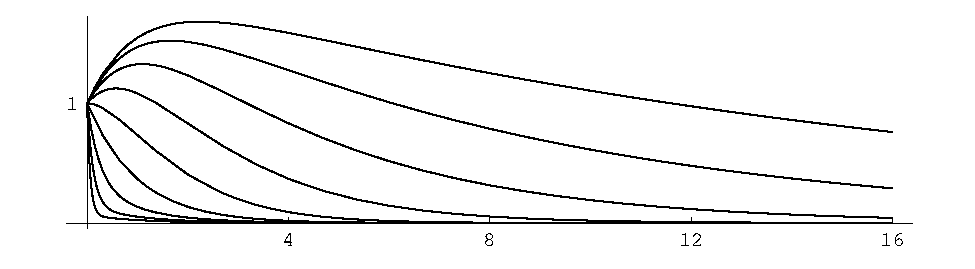
\includegraphics[width=\textwidth]{ode/first_order/range_alpha}
    \end{center}
    \caption{The solution for a range of values of the parameter.}
    \label{figure range alpha}
  \end{figure}

  Consider the solution in the limit as $\alpha \to 0$.
  \begin{align*}
    \lim_{\alpha \to 0} y(x)
    &= \lim_{\alpha \to 0} \frac{1}{\alpha - 1} \left( \e^{-x} 
      + (\alpha-2) \e^{- \alpha x} \right) \\
    &= 2 - \e^{-x}
  \end{align*}
  In the limit as $\alpha \to \infty$ we have,
  \begin{align*}
    \lim_{\alpha \to \infty} y(x)
    &= \lim_{\alpha \to \infty} \frac{1}{\alpha - 1} \left( \e^{-x} 
      + (\alpha-2) \e^{- \alpha x} \right) \\
    &= \lim_{\alpha \to \infty} \frac{\alpha-2}{\alpha - 1} 
    \e^{- \alpha x} \\
    &= \begin{cases}
      1 & \mathrm{for}\ x = 0, \\
      0 & \mathrm{for}\ x > 0.
    \end{cases}
  \end{align*}
  This behavior is shown in Figure~\ref{alpha_0_alpha_inf}.  The first graph
  plots the solutions for $\alpha = 1/128, 1/64, \ldots,1$.
  The second graph plots the solutions for 
  $\alpha = 1,2,\ldots,128$.

  \begin{figure}[tb!]
    \begin{center}
      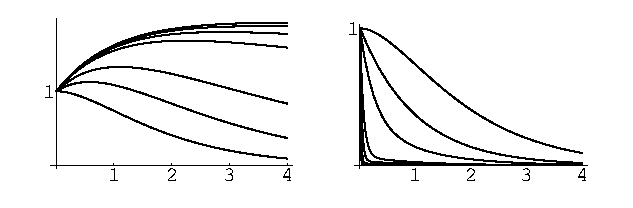
\includegraphics[width=0.7\textwidth]{ode/first_order/alpha_0_alpha_inf}
    \end{center}
    \caption{The solution for limiting values of the parameter.}
    \label{alpha_0_alpha_inf}
  \end{figure}
\end{Solution}







%% Taylor series about origin
\begin{Solution} 
  \label{solution dwdz + 1 1-z w}
  We substitute $w = \sum_{n=0}^\infty a_n z^n$ into the equation 
  $\frac{\dd w}{\dd z} + \frac{1}{1-z} w = 0$.
  \begin{gather*}
    \frac{\dd}{\dd z} \sum_{n=0}^\infty a_n z^n 
    + \frac{1}{1-z}\sum_{n=0}^\infty a_n z^n = 0 \\
    (1-z)\sum_{n=1}^\infty n a_n z^{n-1} + \sum_{n=0}^\infty a_n z^n = 0 \\
    \sum_{n=0}^\infty (n+1) a_{n+1} z^n - \sum_{n=0}^\infty n a_n z^n
    + \sum_{n=0}^\infty a_n z^n = 0 \\
    \sum_{n=0}^\infty \left( (n+1) a_{n+1} - (n-1) a_n \right) z^n = 0
  \end{gather*}
  Equating powers of $z$ to zero, we obtain the relation,
  \[
  a_{n+1} = \frac{n-1}{n+1} a_n.
  \]
  $a_0$ is arbitrary.  We can compute the rest of the coefficients from the 
  recurrence relation.
  \begin{align*}
    &a_1 = \frac{-1}{1} a_0 = -a_0 \\
    &a_2 = \frac{0}{2} a_1 = 0
  \end{align*}
  We see that the coefficients are zero for $n \geq 2$. Thus the Taylor
  series expansion, (and the exact solution),  is
  \[ 
  \boxed{
    w = a_0(1-z).
    } 
  \]
  The radius of convergence of the series in infinite.  The nearest singularity
  of $\frac{1}{1-z}$ is at $z=1$.  Thus we see the radius of convergence can
  be greater than the distance to the nearest singularity of the coefficient 
  function, $p(z)$.
\end{Solution}








\solutions{

  %%-----------------------------------------------------------------------------
  \begin{large}
    \noindent
    \textbf{Exact Equations}
  \end{large}




  \begin{Solution}
    \label{solution dydx=xxyyx}
    \begin{enumerate}
      %%
      %%
    \item
      \[
      \frac{\dd y}{\dd x} = \frac{ x^2 + x y + y^2 }{ x^2 }
      \]
      Since the right side is a homogeneous function of order zero, this is a 
      homogeneous differential equation.  We make the change of variables
      $u = y / x$ and then solve the differential equation for $u$.
      \begin{gather*}
        x u' + u = 1 + u + u^2 \\
        \frac{ \dd u }{ 1 + u^2 } = \frac{ \dd x }{ x } \\
        \arctan(u) = \ln |x| + c \\
        u = \tan( \ln(|c x|) ) \\
        \boxed{
          y = x \tan( \ln(|c x|) )
          }
      \end{gather*}
      %%
      %%
    \item
      \[
      (4y-3x) \,\dd x + (y-2x) \,\dd y = 0
      \]
      Since the coefficients are homogeneous functions of order one, this is a 
      homogeneous differential equation.  We make the change of variables
      $u = y / x$ and then solve the differential equation for $u$.
      \begin{gather*}
        \left( 4 \frac{y}{x} - 3 \right) \,\dd x 
        + \left( \frac{y}{x} - 2 \right) \,\dd y = 0 \\
        (4 u - 3) \,\dd x + (u - 2)(u \,\dd x + x \,\dd u) = 0 \\
        (u^2 + 2 u - 3) \,\dd x + x (u - 2) \,\dd u  = 0 \\
        \frac{\dd x}{x} + \frac{u - 2}{(u+3)(u-1)} \,\dd u = 0 \\
        \frac{\dd x}{x} 
        + \left( \frac{5/4}{u+3} - \frac{1/4}{u-1} \right) \,\dd u = 0 \\
        \ln(x) + \frac{5}{4} \ln(u+3) - \frac{1}{4} \ln(u-1) = c \\
        \frac{ x^4 (u+3)^5 }{ u-1 } = c \\
        \frac{ x^4 (y/x + 3)^5 }{ y/x - 1 } = c \\
        \boxed{
          \frac{ (y + 3 x)^5 }{ y - x } = c
          }
      \end{gather*}
    \end{enumerate}
  \end{Solution}








  \begin{Solution}
    \label{solution dydx=axbybxcy}
    \begin{enumerate}
      %%
      %%
    \item
      \[
      (3x^2-2xy+2) \,\dd x+(6y^2-x^2+3) \,\dd y = 0
      \]
      We check if this form of the equation, $P \,\dd x + Q \,\dd y = 0$, is exact.
      \[
      P_y = - 2 x, \qquad Q_x = -2 x
      \]
      Since $P_y = Q_x$, the equation is exact.  Now we find the primitive
      $u(x,y)$ which satisfies 
      \[
      \dd u = (3x^2-2xy+2) \,\dd x+(6y^2-x^2+3) \,\dd y.
      \]
      The primitive satisfies the partial differential equations
      \begin{equation}
        \label{ux=P,uy=Q}
        u_x = P, \quad u_y = Q.
      \end{equation}
      We integrate the first equation of~\ref{ux=P,uy=Q} to determine $u$ up 
      to a function of integration.
      \begin{gather*}
        u_x = 3 x^2 - 2 x y + 2 \\
        u = x^3 - x^2 y + 2 x + f(y)
      \end{gather*}
      We substitute this into the second equation of~\ref{ux=P,uy=Q} to determine
      the function of integration up to an additive constant.
      \begin{gather*}
        -x^2 + f'(y) = 6 y^2 - x^2 + 3 \\
        f'(y) = 6 y^2 + 3 \\
        f(y) = 2 y^3 + 3 y
      \end{gather*}
      The solution of the differential equation is determined by the 
      implicit equation $u = c$.
      \[
      \boxed{
        x^3 - x^2 y + 2 x + 2 y^3 + 3 y = c
        }
      \]
      %%
      %%
    \item
      \begin{gather*}
        \frac{\dd y}{\dd x} = - \frac{ax+by}{bx+cy} \\
        ( a x + b y ) \,\dd x + ( b x + c y ) \,\dd y = 0
      \end{gather*}
      We check if this form of the equation, $P \,\dd x + Q \,\dd y = 0$, is exact.
      \[
      P_y = b, \qquad Q_x = b
      \]
      Since $P_y = Q_x$, the equation is exact.  Now we find the primitive
      $u(x,y)$ which satisfies 
      \[
      \dd u = ( a x + b y ) \,\dd x + ( b x + c y ) \,\dd y
      \]
      The primitive satisfies the partial differential equations
      \begin{equation}
        \label{ux=P,uy=Q2}
        u_x = P, \quad u_y = Q.
      \end{equation}
      We integrate the first equation of~\ref{ux=P,uy=Q2} to determine $u$ up 
      to a function of integration.
      \begin{gather*}
        u_x = a x + b y \\
        u = \frac{1}{2} a x^2 + b x y + f(y)
      \end{gather*}
      We substitute this into the second equation of~\ref{ux=P,uy=Q2} to determine
      the function of integration up to an additive constant.
      \begin{gather*}
        b x + f'(y) = b x + c y \\
        f'(y) = c y \\
        f(y) = \frac{1}{2} c y^2
      \end{gather*}
      The solution of the differential equation is determined by the 
      implicit equation $u = d$.
      \[
      \boxed{
        a x^2 + 2 b x y + c y^2 = d
        }
      \]
    \end{enumerate}
  \end{Solution}










  \begin{Solution}
    \label{solution dydx = 1-2x y2}
    Note that since these equations are nonlinear, we cannot predict where the 
    solutions will be defined from the equation alone.
    \begin{enumerate}
      %%
      %%
    \item
      This equation is separable.  We integrate to get the general solution.
      \begin{gather*}
        \frac{\dd y}{\dd x} = (1-2x) y^2 \\
        \frac{\dd y}{y^2} = (1 - 2 x) \,\dd x \\
        - \frac{1}{y} = x - x^2 + c \\
        y = \frac{1}{x^2 - x - c}
      \end{gather*}
      Now we apply the initial condition.
      \begin{gather*}
        y(0) = \frac{1}{-c} = - \frac{1}{6} \\
        y = \frac{1}{x^2 - x - 6} \\
        \boxed{
          y = \frac{1}{(x+2)(x-3)}
          }
      \end{gather*}
      The solution is defined on the interval $(-2 \ldots 3)$.
      %%
      %%
    \item
      This equation is separable.  We integrate to get the general solution.
      \begin{gather*}
        x \,\dd x + y \e^{-x} \,\dd y = 0 \\
        x \e^x \,\dd x + y \,\dd y = 0 \\
        (x - 1) \e^x + \frac{1}{2} y^2 = c \\
        y = \sqrt{ 2 ( c + (1-x) \e^x ) }
      \end{gather*}
      We apply the initial condition to determine the constant of integration.
      \begin{gather*}
        y(0) = \sqrt{ 2 (c + 1) }= 1 \\
        c = - \frac{1}{2} \\
        \boxed{
          y = \sqrt{ 2 (1-x) \e^x - 1 }
          }
      \end{gather*}
      The function $2(1-x) \e^x - 1$ is plotted in Figure~\ref{21xex1}.  We see that
      the argument of the square root in the solution is non-negative only on 
      an interval about the origin.  Because $2 (1-x) \e^x - 1 == 0$ is a mixed
      algebraic / transcendental equation, we cannot solve it analytically.  The
      solution of the differential equation is defined on the interval
      $(-1.67835 \ldots 0.768039)$.

      \begin{figure}[tb!]
        \begin{center}
          \includegraphics[width=0.25\textwidth]{ode/first_order/21xex1}
        \end{center}
        \caption{The function.}
        \label{21xex1}
      \end{figure}
    \end{enumerate}
  \end{Solution}










  %% (4 y - x) y' - (9 x^2 + y - 1) = 0.
  \begin{Solution}
    \label{solution 4yxy9x2y10}
    \begin{enumerate}
      %%
      %%
    \item
      We consider the differential equation,
      \[
      (4 y - x) y' - (9 x^2 + y - 1) = 0.
      \]
      \begin{gather*}
        P_y = \frac{\partial}{\partial y} \left( 1 - y - 9 x^2 \right) = -1 \\
        Q_x = \frac{\partial}{\partial x} \left( 4 y - x \right) = -1
      \end{gather*}
      This equation is exact.  It is simplest to solve the equation by rearranging
      terms to form exact derivatives.
      \begin{gather*}
        4 y y' - x y' - y + 1 - 9 x^2 = 0 \\
        \frac{\dd}{\dd x} \left[ 2 y^2 - x y \right] + 1 - 9 x^2 = 0 \\
        2 y^2 - x y + x - 3 x^3 + c = 0 \\
        \boxed{
          y = \frac{1}{4} \left( x \pm \sqrt{x^2 - 8 ( c + x - 3 x^3 ) } \right)
          }
      \end{gather*}
      %%
      %%
    \item
      We consider the differential equation,
      \[
      (2 x - 2 y) y' + (2 x + 4 y) = 0.
      \]
      \begin{gather*}
        P_y = \frac{\partial}{\partial y} \left( 2 x + 4 y \right) = 4 \\
        Q_x = \frac{\partial}{\partial x} \left( 2 x - 2 y \right) = 2
      \end{gather*}
      Since $P_y \neq Q_x$, this is not an exact equation.
    \end{enumerate}
  \end{Solution}










  %% y^2 \sin t + y f(t) \frac{\dd y}{\dd t} = 0
  \begin{Solution}
    \label{solution y2 sin t + y f dydt}
    Recall that the differential equation
    \[
    P(x, y) + Q(x, y) y' = 0
    \]
    is exact if and only if $P_y = Q_x$.
    For Equation~\ref{eqn_y2_sint}, this criterion is 
    \begin{gather*}
      2 y \sin t = y f'(t) \\
      f'(t) = 2 \sin t \\
      \boxed{
        f(t) = 2(a - \cos t).
        }
    \end{gather*}
    In this case, the differential equation is
    \[
    y^2 \sin t + 2 y y' (a - \cos t) = 0.
    \]
    We can integrate this exact equation by inspection.
    \begin{gather*}
      \frac{\dd}{\dd t} \left( y^2 (a - \cos t) \right) = 0 \\
      y^2 (a - \cos t) = c \\
      \boxed{
        y = \pm \frac{c}{ \sqrt{ a - \cos t } }
        }
    \end{gather*}
  \end{Solution}









  %%-----------------------------------------------------------------------------
  \begin{large}
    \noindent
    \textbf{The First Order, Linear Differential Equation}
  \end{large}





  %% y' + \frac{y}{\sin x} = 0. 
  \begin{Solution}
    \label{solution y + y / sin x}
    Consider the differential equation
    \[ 
    y' + \frac{y}{\sin x} = 0. 
    \]
    We use Equation~\ref{first order linear homogeneous} to determine 
    the solution.
    \begin{gather*}
      y = c \e^{ \int -1/\sin x \,\dd x } 
      \\
      y = c \e^{ - \ln | \tan (x/2) | } 
      \\
      y = c \left| \cot \left( \frac{x}{2} \right) \right| 
      \\
      \boxed{ 
        y = c \cot \left( \frac{x}{2} \right)
        } 
    \end{gather*}
  \end{Solution}












  %%-----------------------------------------------------------------------------
  \begin{large}
    \noindent
    \textbf{Initial Conditions}
  \end{large}







  %%-----------------------------------------------------------------------------
  \begin{large}
    \noindent
    \textbf{Well-Posed Problems}
  \end{large}






  %% t \frac{\dd y}{\dd t} + A y = 1 + t^2
  \begin{Solution}
    \label{solution t dydt + A y}
    First we write the differential equation in the standard form.
    \[
    \frac{\dd y}{\dd t} + \frac{A}{t} y = \frac{1}{t} + t, \quad t > 0
    \]
    We determine the integrating factor.
    \[
    I(t) = \e^{\int A / t \,\dd t} = \e^{A \ln t} = t^A
    \]
    We multiply the differential equation by the
    integrating factor and integrate.
    \begin{gather*}
      \frac{\dd y}{\dd t} + \frac{A}{t} y = \frac{1}{t} + t 
      \\
      \frac{\dd}{\dd t} \left( t^A y \right) = t^{A-1} + t^{A+1} 
      \\
      t^A y = \begin{cases}
        \frac{t^A}{A} + \frac{t^{A+2}}{A+2} + c, &A \neq 0, -2 
        \\
        \ln t + \frac{1}{2} t^2 + c, &A = 0 
        \\
        - \frac{1}{2} t^{-2} + \ln t + c, &A = -2
      \end{cases} 
      \\
      y = \begin{cases}
        \frac{1}{A} + \frac{t^2}{A+2} + c t^{-A}, &A \neq -2 
        \\
        \ln t + \frac{1}{2} t^2 + c, &A = 0 
        \\
        - \frac{1}{2} + t^2 \ln t + c t^2, &A = -2
      \end{cases}
    \end{gather*}
    For positive $A$, the solution is bounded at the origin only for $c = 0$.
    For $A = 0$, there are no bounded solutions.
    For negative $A$, the solution is bounded there for any value of $c$ and 
    thus we have a one-parameter family of solutions.

    In summary, the solutions which are bounded at the origin are:
    \[
    \boxed{
      y =
      \begin{cases}
        \frac{1}{A} + \frac{t^2}{A+2}, &A > 0 
        \\
        \frac{1}{A} + \frac{t^2}{A+2} + c t^{-A}, &A < 0,\ A \neq -2 
        \\
        - \frac{1}{2} + t^2 \ln t + c t^2, &A = -2
      \end{cases}
      }
    \]
  \end{Solution}






  %%-----------------------------------------------------------------------------
  \begin{large}
    \noindent
    \textbf{Equations in the Complex Plane}
  \end{large}




  %% Classify the singular points of the following first order differential
  \begin{Solution}  
    \label{solution dwdz + sin z z w}

    $\phantom{a}$   %% Used to force a new paragraph.

    \begin{enumerate}
      %%
    \item Consider the equation $w' + \frac{\sin z}{z} w = 0$.  
      The point $z=0$ is the only point we need to examine in the finite plane.
      Since $\frac{\sin z}{z}$ has a removable singularity at $z=0$, there are 
      no singular points in the finite plane.
      The substitution $z = \frac{1}{\zeta}$ yields the equation
      \[ 
      u' - \frac{\sin(1/\zeta)}{\zeta}u = 0.
      \]
      Since $\frac{\sin(1/\zeta)}{\zeta}$ has an essential singularity at 
      $\zeta = 0$, the point at infinity is an irregular singular point of the 
      original differential equation.
      %%
    \item Consider the equation $w' + \frac{1}{z-3} w = 0$.
      Since $\frac{1}{z-3}$ has a simple pole at $z=3$, the differential equation
      has a regular singular point there.  Making the substitution 
      $z = 1/\zeta$, $w(z)=u(\zeta)$
      \begin{gather*}
        u' - \frac{1}{\zeta^2(1/\zeta-3)} u  = 0 \\
        u' - \frac{1}{\zeta(1-3\zeta)} u = 0.
      \end{gather*}
      Since this equation has a simple pole at $\zeta = 0$, the original equation 
      has a regular singular point at infinity.
      %%
    \item Consider the equation $w' + z^{1/2} w = 0$.
      There is an irregular singular point at $z = 0$.  With the substitution
      $z = 1/\zeta$, $w(z) = u(\zeta)$,
      \begin{gather*}
        u' - \frac{\zeta^{-1/2}}{\zeta^2} u = 0 \\
        u' - \zeta^{-5/2} u = 0.
      \end{gather*}
      We see that the point at infinity is also an irregular singular point
      of the original differential equation.
    \end{enumerate}
  \end{Solution}







  %% Expand irregular singular point in a Frobenius series.
  \begin{Solution} 
    \label{solution dwdz z-2 w}
    We start with the equation
    \[ 
    w' + z^{-2}w = 0.
    \]
    Substituting $w = z^\lambda \sum_{n=0}^\infty a_n z^n$, $a_0 \neq 0$ yields
    \begin{gather*}
      \frac{\dd}{\dd z} \left(z^\lambda \sum_{n=0}^\infty a_n z^n\right) + 
      z^{-2}z^\lambda \sum_{n=0}^\infty a_n z^n = 0 \\
      \lambda z^{\lambda-1} \sum_{n=0}^\infty a_n z^n 
      + z^\lambda \sum_{n=1}^\infty n a_n z^{n-1}
      + z^\lambda \sum_{n=0}^\infty a_n z^{n-2} = 0
    \end{gather*}
    The lowest power of $z$ in the expansion is $z^{\lambda-2}$.  The 
    coefficient of this term is $a_0$.  Equating powers of $z$ demands that
    $a_0 = 0$ which contradicts our initial assumption that it was nonzero.
    Thus we cannot find a $\lambda$ such that the solution can be expanded
    in the form,
    \[ 
    w = z^\lambda \sum_{n=0}^\infty a_n z^n, \qquad a_0 \neq 0.
    \]
  \end{Solution}

  

\raggedbottom
}
%%=============================================================================
\pagebreak
\flushbottom
\section{Quiz}


\begin{QuizProblem}
  \label{quiz problem general solution first order}
  What is the \textit{general solution} of a first order 
  differential equation?

  \quizsolution{general solution first order}
\end{QuizProblem}


\begin{QuizProblem}
  \label{quiz problem first order exact separable}
  Write a statement about the functions $P$ and $Q$ to make the following 
  statement correct.

  The first order differential equation
  \[
  P(x, y) + Q(x, y) \frac{\dd y}{\dd x} = 0
  \]
  is exact if and only if $\underline{\phantom{P_y = Q_x}}$.
  It is separable if $\underline{\phantom{P = P(x) and Q = Q(y)}}$.

  \quizsolution{first order exact separable}
\end{QuizProblem}


\begin{QuizProblem}
  \label{quiz problem y' + p y = f}
  Derive the general solution of
  \[
  \frac{\dd y}{\dd x} + p(x) y = f(x).
  \]

  \quizsolution{y' + p y = f}
\end{QuizProblem}


\begin{QuizProblem}
  \label{quiz problem y' = y + y2}
  Solve $y' = y - y^2$.

  \quizsolution{y' = y + y2}
\end{QuizProblem}








\raggedbottom
%%=============================================================================
\pagebreak
\flushbottom
\section{Quiz Solutions}


\begin{QuizSolution}
  \label{quiz solution general solution first order}
  The general solution of a first order differential equation is a 
  one-parameter family of functions which satisfies the equation.
\end{QuizSolution}


\begin{QuizSolution}
  \label{quiz solution first order exact separable}
  The first order differential equation
  \[
  P(x, y) + Q(x, y) \frac{\dd y}{\dd x} = 0
  \]
  is exact if and only if $P_y = Q_x$.
  It is separable if $P = P(x)$ and $Q = Q(y)$.
\end{QuizSolution}


\begin{QuizSolution}
  \label{quiz solution y' + p y = f}
  \[
  \frac{\dd y}{\dd x} + p(x) y = f(x)
  \]
  We multiply by the integrating factor 
  $\mu(x) = \exp(P(x)) = \exp\left( \int p(x) \,\dd x \right)$, and integrate.
  \begin{gather*}
    \frac{\dd y}{\dd x} \e^{P(x)} + p(x) y \e^{P(x)} = \e^{P(x)} f(x) 
    \\
    \frac{\dd}{\dd x} \left( y \e^{P(x)} \right) = \e^{P(x)} f(x) 
    \\
    y \e^{P(x)} = \int \e^{P(x)} f(x)\,\dd x + c 
    \\
    y = \e^{-P(x)} \int \e^{P(x)} f(x)\,\dd x + c \e^{-P(x)}
  \end{gather*}
\end{QuizSolution}


\begin{QuizSolution}
  \label{quiz solution y' = y + y2}
  $y' = y - y^2$ is separable.
  \begin{gather*}
    y' = y - y^2 
    \\
    \frac{y'}{y - y^2} = 1 
    \\
    \frac{y'}{y} - \frac{y'}{y - 1} = 1 
    \\
    \ln y - \ln(y - 1) = x + c 
    \\
    \intertext{We do algebraic simplifications and rename the constant 
      of integration to write the solution in a nice form.}
    \frac{y}{y-1} = c \e^x 
    \\
    y = (y - 1) c \e^x 
    \\
    y = \frac{-c \e^x}{1 - c \e^x} 
    \\
    y = \frac{\e^x}{\e^x - c} 
    \\
    y = \frac{1}{1 - c \e^{-x}} 
  \end{gather*}
\end{QuizSolution}










\raggedbottom
